%%%%%%%%%%%%%%%%%%%%%%%%%%%%%%%%%%%%%%%%%
% Short Sectioned Assignment LaTeX Template Version 1.0 (5/5/12)
% This template has been downloaded from: http://www.LaTeXTemplates.com
% Original author:  Frits Wenneker (http://www.howtotex.com)
% License: CC BY-NC-SA 3.0 (http://creativecommons.org/licenses/by-nc-sa/3.0/)
%%%%%%%%%%%%%%%%%%%%%%%%%%%%%%%%%%%%%%%%%

% \documentclass[paper=a4, fontsize=11pt]{scrartcl} % A4 paper and 11pt font size
\documentclass[11pt, a4paper, fleqn]{report}
\usepackage[T1]{fontenc} % Use 8-bit encoding that has 256 glyphs
\usepackage[utf8]{inputenc}
\usepackage{listings} % para insertar código con formato similar al editor
\usepackage{color}
\usepackage{subcaption}

\definecolor{dkgreen}{rgb}{0,0.6,0}
\definecolor{gray}{rgb}{0.5,0.5,0.5}
\definecolor{mauve}{rgb}{0.58,0,0.82}

\lstset{frame=tb,
	language=python,
	aboveskip=3mm,
	belowskip=3mm,
	showstringspaces=false,
	columns=flexible,
	basicstyle={\small\ttfamily},
	numbers=none,
	numberstyle=\tiny\color{gray},
	keywordstyle=\color{blue},
	commentstyle=\color{dkgreen},
	stringstyle=\color{mauve},
	breaklines=true,
	breakatwhitespace=true,
	tabsize=4
}
\usepackage[spanish, es-tabla]{babel} % Selecciona el español para palabras introducidas automáticamente, p.ej. "septiembre" en la fecha y especifica que se use la palabra Tabla en vez de Cuadro
\usepackage{url} % ,href} %para incluir URLs e hipervínculos dentro del texto (aunque hay que instalar href)
\usepackage{graphics,graphicx, float} %para incluir imágenes y colocarlas
\usepackage[gen]{eurosym} %para incluir el símbolo del euro
\usepackage{cite} %para incluir citas del archivo <nombre>.bib
\usepackage{enumerate}
\usepackage{hyperref}
\usepackage{graphicx}
\usepackage{tabularx}
\usepackage{booktabs}
\usepackage{amsmath}
\graphicspath{{././img}}
\usepackage[table,xcdraw]{xcolor}
\hypersetup{
	colorlinks=true,	% false: boxed links; true: colored links
	linkcolor=blue,  	% color of internal links
	urlcolor=cyan		% color of external links
}
\renewcommand{\familydefault}{\sfdefault}
\usepackage{fancyhdr} % Custom headers and footers
\pagestyle{fancyplain} % Makes all pages in the document conform to the custom headers and footers
\fancyhead[L]{} % Empty left header
\fancyhead[C]{} % Empty center header
\fancyhead[R]{Antonio Manuel Fresneda} % My name
\fancyfoot[L]{} % Empty left footer
\fancyfoot[C]{} % Empty center footer
\fancyfoot[R]{\thepage} % Page numbering for right footer
%\renewcommand{\headrulewidth}{0pt} % Remove header underlines
\renewcommand{\footrulewidth}{0pt} % Remove footer underlines
\setlength{\headheight}{13.6pt} % Customize the height of the header
\decimalpoint
\definecolor{gray75}{gray}{0.75}
\newcommand{\hsp}{\hspace{20pt}}

\setcounter{secnumdepth}{4}

\begin{document}
	\begin{titlepage}
\newlength{\centeroffset}
\setlength{\centeroffset}{-0.5\oddsidemargin}
\addtolength{\centeroffset}{0.5\evensidemargin}
\thispagestyle{empty}

\noindent\hspace*{\centeroffset}\begin{minipage}{\textwidth}

\centering

\includegraphics[width=0.9\textwidth]{logos/logo_ugr.jpg}\\[1.4cm]

\textsc{ \Large TRABAJO FIN DE GRADO\\[0.2cm]}
\textsc{ GRADO EN INGENIERIA INFORMATICA}\\[1cm]

{\Huge\bfseries   Titulo\\}
\noindent\rule[-1ex]{\textwidth}{3pt}\\[3.5ex]
{\large\bfseries }
\end{minipage}

\vspace{2.5cm}
\noindent\hspace*{\centeroffset}
\begin{minipage}{\textwidth}
\centering

\textbf{Autor}\\ {Antonio Manuel Fresneda Rodríguez}\\[2.5ex]
\textbf{Director}\\ {Salvador García López }\\[2cm]

\includegraphics[width=0.3\textwidth]{logos/etsiit_logo.png}\\[0.1cm]
\textsc{Escuela Técnica Superior de Ingenierías Informática y de Telecomunicación}\\
\textsc{---}\\
Granada, mes de año
\end{minipage}
\end{titlepage}

	\thispagestyle{empty}

\begin{center}
{\large\bfseries Análisis de la intención de emprendimiento a través de una recogida de datos por encuestas mediante técnicas de preprocesamiento de datos y aprendizaje automático.}\\
\end{center}
\begin{center}
Antonio Manuel Fresneda Rodríguez.\\
\end{center}

%\vspace{0.7cm}

\vspace{0.5cm}
\noindent{\textbf{Palabras clave}: \textit{intención emprendedora}, \textit{aprendizaje automático}, \textit{clasificación ordinal}, \textit{clasificación multi-etiqueta}, \textit{regresión}, \textit{Python}
\vspace{0.7cm}

\noindent{\textbf{Resumen}\\
	\linebreak 
	Para que un país sea sólido económicamente, necesita empresas productivas, ya que son las que crean puestos de trabajo e impulsan el desarrollo económico.\\
	Por este motivo, detectar a aquellas personas que son capaces de crear nuevas empresa y promover que estas sean capaces de emprender y facilitar el acceso a recursos y asesoramiento necesarios puede ser un factor importante de cara al crecimiento económico de un país.\\
	La intención emprendedora se puede definir como el estado mental que provoca una atención, experiencia y acción hacia un concepto de negocio, asumiendo que esa persona no reacciona de forma automática antes los estímulos del medio, sino que procesa la información que le rodea (Bird. 1998).\\
	\linebreak
	Resolver este tipo de problemas usando técnicas clásicas puede no ser la mejor opción, ya que puede llegar a ser muy costoso en tiempo y recursos. Con el objetivo de facilitar este tipo de problemas nació el Aprendizaje Automático.\\
	El Aprendizaje Automático hace uso de unos \textbf{datos} y construye un \textbf{modelo} capaz de realizar \textbf{predicciones} tanto de los datos que ha usado como de datos nuevos.\\
	Este campo ha sufrido una gran evolución en estos últimos años, donde se han propuesto nuevos problemas, modelos y metodología, aumentando la cantidad de problemas que pueden ser resueltos.\\
	\linebreak
	Este trabajo hace uso de técnicas de Aprendizaje Automático y de unos \textbf{datos} recogidos sobre un conjunto de la población española y ecuatoriana para intentar predecir si una persona va a tener una intención emprendedora y cuales son los factores más importantes para que una persona tome este tipo de decisiones.
\cleardoublepage

\begin{center}
	{\large\bfseries Analysis of entrepreneurial intention through data collected by surveys using data preprocessing techniques and Machine Learning }\\
\end{center}
\begin{center}
	Antonio Manuel Fresneda Rodríguez\\
\end{center}
\vspace{0.5cm}
\noindent{\textbf{Keywords}: \textit{entrepreneurial intention}, \textit{machine learning}, \textit{ordinal classification}, \textit{multi-label clasification}, \textit{regression}, \textit{Python}
\vspace{0.7cm}

\noindent{\textbf{Abstract}\\
\linebreak
To keep a country solid economically, it will need profitable companies, as these are in charge of creating job posts and pushing the economic growth.\\
For these reasons, detecting people capable of creating new companies and helping them to get the resources and advice, can be important for the economic growth of a country.
Entrepreneurial intention is the mental state of mind that precedes action and directs attention toward entrepreneurial behaviors such as starting a new business. This person will use all the information around him/her and will process it to get the best decision, instead of reacting automatically to the stimuli (Bird 1998).\\
\linebreak
Solving this kind of problem using classic techniques may not be the best choice, as this can be time and resource-intensive. The goal of  Machine Learning is to ease this kind of problem. This approach will use data to build a mathematical model that will predict the data used to create the model and, most important, new data that the model hasn't used.
This field has evolved significantly during the last years, proposing new problems, models, and methodology.\\
\linebreak
This work will use Machine Learning techniques and data collected from Spanish and Ecuadorian people to find the entrepreneurial intention of a person and which are the key factors that make that choice.
\cleardoublepage
\chapter*{}
\thispagestyle{empty}

\noindent\rule[-1ex]{\textwidth}{2pt}\\[4.5ex]

Yo, \textbf{Antonio Manuel Fresneda Rodríguez}, alumno de la titulación Ingeniería Informática de la \textbf{Escuela Técnica Superior de Ingenierías Informática y de Telecomunicación de la Universidad de Granada}, con DNI 77447672W, autorizo la ubicación de la siguiente copia de mi Trabajo Fin de Grado en la biblioteca del centro para que pueda ser consultada por las personas que lo deseen.
\vspace{6cm}

\noindent Fdo: Antonio Manuel Fresneda Rodríguez
\vspace{2cm}
\begin{flushright}
	Granada a 17 de Noviembre de 2021 .
\end{flushright}

\cleardoublepage
\thispagestyle{empty}

\noindent\rule[-1ex]{\textwidth}{2pt}\\[4.5ex]

D. \textbf{Salvador García López}, Profesor del Área de Computación y Sistemas Inteligentes del Departamento de Ciencias de la Computación e Inteligencia Artificial de la Universidad de Granada.

\vspace{0.5cm}

\textbf{Informo:}

\vspace{0.5cm}

Que el presente trabajo, titulado \textit{\textbf{ Análisis de la intención de emprendimiento a través de una recogida de datos por encuestas mediante técnicas de preprocesamiento de datos y aprendizaje automático}},
ha sido realizado bajo mi supervisión por \textbf{Antonio Manuel Fresneda Rodríguez}, y autorizo la defensa de dicho trabajo ante el tribunal
que corresponda.

\vspace{0.5cm}

Y para que conste, expiden y firman el presente informe en Granada a Noviembre de 2021.

\vspace{1cm}

\textbf{El/la director(a)/es: }

\vspace{5cm}

\noindent \textbf{Salvador García López}
\pagebreak
\section*{Agradecimientos}
Me gustaría comenzar esta sección agradeciendo a mis padres el esfuerzo y la oportunidad que ellos no tuvieron para disfrutar de una educación universitaria. Muchas gracias por todo y os estoy realmente agradecido. \\
A mis hermanas, que son muy importantes para mi y que siempre han estado ahí para apoyarme y de vez en cuando para cabrearme también.
A toda mi familia, gracias abuela, abuelo, tíos, tías, primos, primas os quiero mucho y sois el pilar más importante de mi vida.\\
\linebreak
No me quiero olvidar tampoco de aquellos profesores que han formado parte en mi educación, desde la secundaria, donde creo que en ese momento no llegué a valorar lo importante que era la formación en ingles que estuve recibiendo, hasta todos aquellos docentes que me han dado clase durante todos estos años en la ETSIIT aprendiendo todo lo que me ha llevado a conseguir un trabajo en estas épocas tan complicadas y que me está haciendo muy feliz. Muchas gracias.\\
Una mención aparte para Salva, que me ha propuesto un trabajo muy interesante, me ha ayudado y animado a realizar este trabajo al que le he dedicado un montón de horas en estos meses. Muchas gracias.\\
\linebreak
Agradecer también a todos mis amigos y amigas que he estado haciendo durante todos estos años, muchas gracias por estar siempre ahí y por ser capaces de hacerme desconectar de vez en cuando. 

	\newpage
	\tableofcontents
	\pagebreak

	\chapter{Introducción}
Gracias a la evolución tecnológica que hemos experimentado estos últimos años, y sobre todo a la gigantesca expansión del Internet y a la cantidad de datos generados por dispositivos conectados a la red, ha provocado un enorme interés analizar los datos recogidos.\\
Gracias a esta información es los que nos identifican como posibles compradores de un producto, los que hacen que los coches puedan conducir por si mismos o incluso, ayuden al personal médico detectar una patología a partir de ciertos datos del paciente.\\
\linebreak
Se denomina \textbf{ciencia de datos} a la extracción del conocimiento de una gran cantidad datos mediante el uso del software y de técnicas estadísticas. Este conocimiento puede ser usado para \textbf{predecir} cierta salida en función de los datos, para \textbf{detectar grupos} de datos que tengan características similares, \textbf{explicar} el comportamiento de esos datos, entre otros muchos más casos de uso. \\
\linebreak
En el proyecto que se va a estudiar en las secciones siguientes, trata de responder una serie de cuestiones relacionadas con la \textbf{Intención Emprendedora} de una persona.\\
Se podría definir la Intención Emprendedora de una persona como el estado mental que provoca una atención, experiencia y acción hacia un concepto de negocio (Bird. 1998), asumiendo dicha persona no reacciona de forma automática ante los estímulos del medio, sino que procesa la información que le rodea.
\clearpage
\section{Motivación}
En la economía moderna, las empresas juegan un papel muy importante, ya que son una fuente de empleo y riqueza en las economías modernas. Debido al impacto que pueden tener sobre la economía, se debe de apostar por aquellas personas dispuestas a crear una empresa, asegurando que puedan acceder a los recursos formativos y asesoramiento necesario, ya que puede ser un factor muy importante en el proceso de recuperación económica tras la crisis derivada de la pandemia que ha ocurrido estos últimos años.\\
\linebreak
Con esta idea en mente, el trabajo que se ha realizado en este proyecto busca el detectar si una persona tiene una actitud emprendedora, con el objetivo de detectar a aquellas personas más idóneas y que puedan aprovechar al máximo la información a la que pueden acceder. También busca igualar las posibilidades para aquellas personas que tengan esa actitud, pero es posible que tengan dudas a la hora de emprender, pudiendo asesorar correctamente a estas personas.\\
\linebreak
Además de predecir cual es la intención emprendedora de una persona, es muy importante saber cuales son los factores más influyentes a la hora de detectar este tipo de actitudes en las personas, ya que así se puede trabajar en aquellos factores más relevantes, con el objetivo de incrementar el número de personas dispuestas a emprender, ya que según los datos mostrados en \cite{ie}, menos de un $4\%$ de los recién titulados optan por la creación de empresas en su primer empleo. Esta información podría ser usada para que estos recién graduados y graduadas tengan más fácil el camino del emprendimiento y el de la creación de nuevas empresas.\\
\linebreak
El hacer uso de las técnicas de aprendizaje automático junto con los objetivos que se han mencionado previamente, son factores que han influido a la hora de escoger este trabajo.\\
\linebreak
Todos estos motivos y objetivos relacionados con el problema, han sido las principales motivaciones de resolver e intentar explicar cuales son los factores más influyentes de este problema.
\clearpage
\section{Objetivos}
\label{sec:obj}
A continuación, se enumeran los distintos objetivos que se han puesto a la hora de realizar el trabajo. \\
\linebreak
El primer objetivo que se plantea es el de comprobar si hay conocimiento en el conjunto de datos que se nos ha proporcionado. Probablemente, este sea uno de los pasos más importante a la hora de afrontar este tipo de problemas, ya que puede ocurrir que se hayan cometido errores a la hora de recoger los datos, no se haya recogido una muestra suficientemente grande para resolver el problema o simplemente, no se pueda abordar con estas técnicas. Ejecutar correctamente este paso es clave, ya que detectando estos problemas (entre otros que pueden ocurrir) antes de seguir profundizando, puede evitar invertir tiempo y esfuerzo.\\
\linebreak
Siguiendo con la lista de objetivos de este trabajo era el de comprobar que preguntas (variables del conjunto de entrenamiento) son relevantes y cuales no. Las variables usadas en todo el proceso de KDD han sido recogidas mediante una encuesta. Estas encuestas pueden resultar tediosas cuando se añaden preguntas que son muy poco relevantes, por lo que la posibilidad de re-plantear ciertas preguntas que se han demostrado que no influyen o que los algoritmos no han encontrado puede ser una buena idea, siempre y cuando se analice el porqué esa pregunta es mala, ya que hay que tener en cuenta la posibilidad de que para un modelo una o varias preguntas no sea relevantes, pero en otro  sí que lo sean.\\
\linebreak
Otro punto de mejora sobre la redacción de estas encuestas es el detectar si un cierto campo ha tenido mucha relevancia, podría ser buena idea plantear la posibilidad de, en un futuro, añadir nuevas preguntas relacionadas con ese campo para comprobar si se puede mejorar el rendimiento de los modelos, teniendo en cuenta (obviamente) que se va a trabajar con conjunto de datos distinto, por lo que puede haber ciertas diferencias.\\
\linebreak
El ultimo objetivo que se ha planteado es el de ser capaces de predecir si una persona tiene una actitud emprendedora o no, obteniendo una información muy importante a la hora de mejorar la selección de posibles en una campaña de marketing especializando las ofertas según la intención emprendedora. 
\clearpage
\section{Conocimientos previos y adquiridos}
En esta sección se van a comentar cuales han sido los conocimientos previos a la realización de este trabajo. Durante mis estudios en el grado de Ingeniería Informática me llamó el campo de la inteligencia artificial, debido a la gran cantidad de problemas que usando otro tipo de técnicas no pueden ser resueltos debido al coste en tiempo y recursos que habría que dedicar para resolverlos.\\
Las principales asignaturas que del grado donde adquirí los conocimientos han sido:
\begin{itemize}
	\item \textbf{Aprendizaje Automático:} En esta asignatura aprendí las bases del Machine Learning y cuales son los modelos más usados. entendiendo como funciona e incluso implementando algunos modelos de Aprendizaje Automático.
	\item \textbf{Inteligencia de Negocio:} Esta asignatura tiene un enfoque muy distinto, ya que se centraba más en el estudio de las técnicas necesarias para preparar el conjunto de datos que en el conocimiento profundo de los distintos modelos.
	\item \textbf{Programación Orientada a Objetos:} Todo el uso de clases abstractas, herencia y conceptos básicos sobre este paradigma de programación también ha sido útil para la realización de este trabajo.
\end{itemize}
En todas las asignaturas en las que he trabajado en este tipo de problemas, siempre he trabajado con conjunto de datos que han sido seleccionados por los profesores, aumentando la posibilidad de que se filtrase algunos de los problemas más importantes que puede tener un conjunto de datos obtenidos en bruto.\\
Podría haber buscado un trabajo más fácil, usando unos datos que ya han sido probados con algoritmos de aprendizaje automático y tener la certeza que de una forma u otra, iba a obtener unos resultados buenos siguiendo el mismo proceso que han seguido otras personas que se han enfrentado al problema previamente. Cuando se me propuso este trabajo, en el que podía enfrentarme a un problema nuevo, al que nunca me había enfrentado durante la época de formación en la universidad, la posibilidad de enfrentarme de una manera más "real" a un problema de este tipo, y sobre todo, la oportunidad de aprender nuevos conceptos y técnicas de este campo, fueron razones suficientes por las que decidí realizar este trabajo.\\
\linebreak
Gracias a este trabajo, he podido aprender nuevos tipos de problemas de Machine Learning a los que no me había enfrentado antes, tales como \textbf{clasificación multi-etiqueta} o \textbf{clasificación ordinal}. También he profundizado en estos conocimientos adquiridos, aprendiendo nuevos conceptos y consolidando aquellos que había obtenido cursando estas asignaturas.\\
\clearpage
\section{Estructura de la memoria}
Esta memoria está organizada en distintos capítulos que irán guiando en el desarrollo del trabajo, enfoques usados y cualquier concepto que este relacionado.\\
\linebreak
Se va a comenzar explicando que es el \textit{Machine Learning} y de manera general, conceptos clave que se necesitan tener en cuenta para la comprensión del trabajo. Este capítulo aborda los distintos problemas que se pueden encontrar y como se agrupan los mismos.\\
\linebreak
Después de la explicación de estos conceptos básicos, se va a explicar el problema que se ha abordado en este trabajo, explicando de una forma más específica que tipo de problema es, de donde viene y que elementos lo forman.\\
\linebreak
Explicado los conceptos básicos del problema, se comienza por realizar un análisis de los datos que se han proporcionado. En este sección se explicaran como están formados los datos, y que procesamiento se ha necesitado hacer para que los algoritmos funcionen.
\linebreak
Una vez explicado el problema y el procesamiento previo que se ha realizado, se explican que algoritmos se han usado y cual es la metodología seguida para asegurar unos resultados correctos, evitando caer en las equivocaciones más comunes a la hora de enfrentarse a un problema de este tipo. Esta sección también explicará las distintas formas en las que se han usado para medir el rendimiento de los algoritmos.\\
\linebreak
A continuación, se encuentra un bloque compuesto por varias secciones donde se muestran resultados, análisis de los mismos y variaciones que se han probado y los resultados de las distintas opciones que se han barajado.\\
\linebreak
Mostrado ya los resultados, se continua explicando cual ha sido el proceso software que se ha seguido durante el desarrollo. En esta sección se explicará lenguajes de programación, pautas que se han seguido, herramientas usadas y el proceso de instalación y ejecución del proyecto.\\
\linebreak
Finalmente, se mostrara el bloque de conclusiones y trabajos futuros. Estas secciones finalizaran el proyecto respondiendo a las distintas preguntas que se han hecho durante el desarrollo y valorando si se han cumplido los objetivos propuestos en un inicio.



	\pagebreak

	\chapter{Pre-procesamiento}
\label{sec:pre}
Cualquier problema en ciencia de datos, comienza con un estudio exhaustivo de los datos proporcionados y realizar un \textbf{procesamiento} previo.
Si este paso es omitido, los algoritmos no se comportarán de forma óptima, debido a que van a lidiar con unos datos que tendrán valores perdidos, que no estén normalizados, datos des-balanceados, irrelevantes, entre otras problemas. El objetivo de esta fase, es realizar ciertas transformaciones sobres los datos en bruto filtrando esta información para que los algoritmos no tengan que enfrentarse a estos problemas.
\section{Análisis exploratorio de los datos}

Para comenzar, se empezó leyendo la documentación aportada con los datos, la cual contenía los siguientes campos:
\begin{itemize}
	\item \textbf{Nombre:} Nombre de la característica.
	\item \textbf{Descripción:} Breve resumen explicando el origen de la característica o el enunciado de la pregunta en la encuesta.
	\item \textbf{Valores:} Tipo y/o rango que toma la característica.
\end{itemize}

Esta información es muy útil, ya que aparte de darnos un poco más de conocimiento del objetivo que queremos alcanzar con estos datos, nos da información de algunas características redundantes.

\begin{table}[H]
	\begin{tabular}{|l|l|l|}
		\cline{1-3}
		CF9 & Normalmente es posible reducir... & Respuesta: Verdadera/Falsa.                   \\ \cline{1-3}
		QF9 & Variable creada a partir de CF9.  & Valor 1 si la respuesta es correcta, 0 si no. \\ \cline{1-3}
	\end{tabular}
	\label{tab:columnas_iguales}
	\caption{Comparación de dos características redundantes.}
\end{table}
Como podemos ver, estas dos columnas contienen información redundante, ya que siendo una respuesta de tipo verdadero o falso, tenemos dos columnas con la misma información. Este caso se repite en varios casos, y en todos ellos se ha optado por dejar unicamente la que tiene los valores numéricos.\\
\linebreak
El siguiente paso ha sido el de obtener las columnas que se van a usar como predictores.
La peculiaridad de este conjunto de datos tenemos 7 columnas que van a ser las que los algoritmos tienen que intentar predecir. De estas 7 columnas tenemos 6 de ellas que son de tipo ordinal, almacenando la opinión (en escala Likert) que ha tenido el entrevistado sobre la pregunta en concreto. La ultima de estas columnas es la media de las 6 columnas.\\
A continuación se muestra una tabla con la ocurrencia de cada valor para las columnas que vamos a usar:\\
\linebreak
\begin{figure}[H]
	\centering
	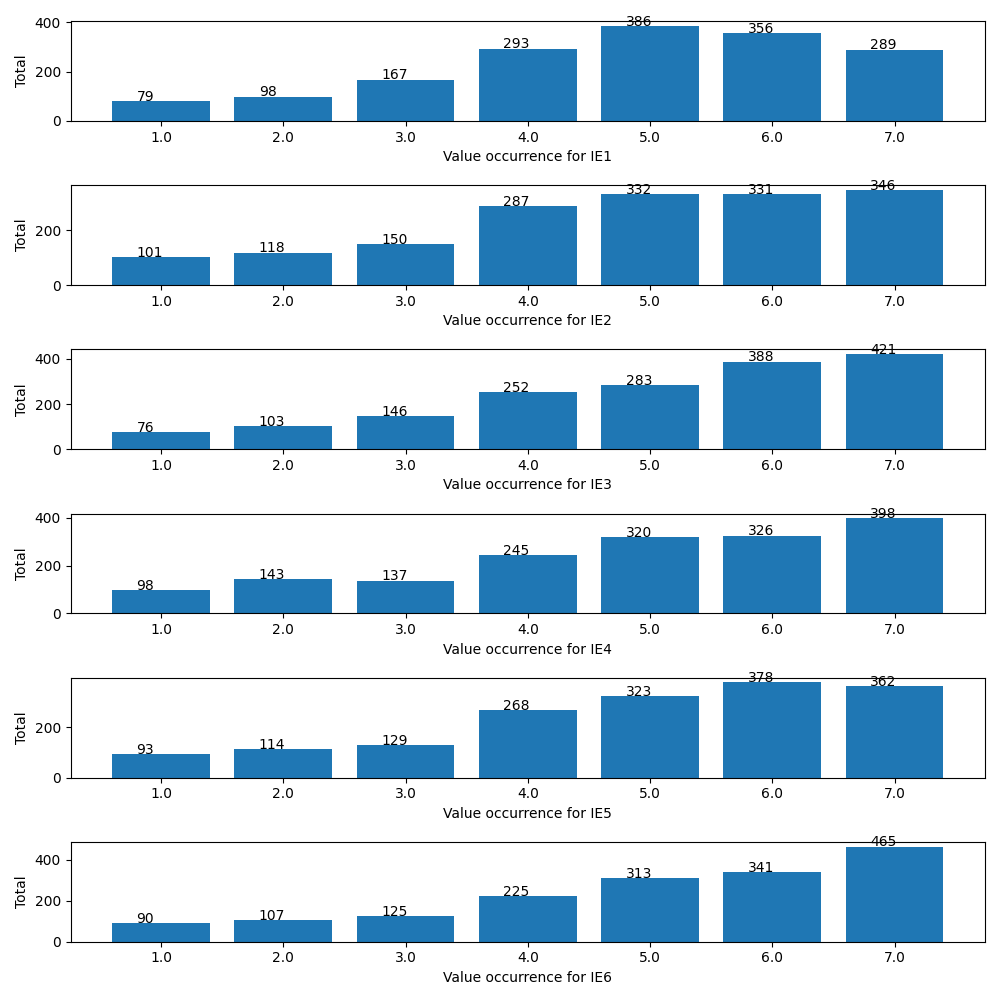
\includegraphics[scale=0.75]{src/value_occurrences.png}
	\caption{Conteo de valores para las columnas usadas como predictores}
	\label{tab:ocurrencia_valores}
\end{figure}
Una vez leída esta documentación y detectados algunos casos de columnas con información redundante, se cargaron los datos y se sacaron una serie de métricas. Estamos ante un conjunto de datos formados por un total de 1672 ejemplos y con 246 características (antes de realizar cualquier tipo de procesamiento), las cuales pueden ser de tipo entero, flotante o categóricas.
\pagebreak
\section{Pre-procesado de datos}
En este paso también se han borrado aquellas columnas las cuales corresponden a respuestas de tipo abierta. Estas características pueden llegar a contener un valor único por cada uno de los ejemplos que tenemos. En un principio, van a ser descartadas, pero en fases siguientes se podría realizar un procesamiento más exhaustivo sobre dicha columna, agrupando ciertos valores y reduciendo así la complejidad. Cabe destacar que esta información no se esta perdiendo totalmente, ya que tenemos en todos los casos una nueva columna la cual contiene si la persona respondió correctamente o no a dicha pregunta. \\
\linebreak
Un caso particular que se detectó en esta fase, fue el de las características \textbf{BFx} y \textbf{BFxAdaptada} (hay un total de 4 columnas de este tipo). Las primeras columnas de este tipo, solo contenían la respuesta las personas que realizaron la entrevista en un único año, mientras que las columnas del segundo tipo contenían la respuestas de los dos años. Antes de eliminar las columnas del primer tipo, se realizo una comprobación para ver si realmente los datos comunes entre las dos columnas eran los mismos para así asegurar que no se están perdiendo datos.
\linebreak
El siguiente paso, ha sido analizar los valores únicos de cada variable, esto nos permitió detectar valores no validos. Se encontró los siguientes casos de valores nó validos:
\begin{itemize}
	\item \textbf{Valores perdidos especificados como espacios:} Si no procesamos estos valores, el algoritmo puede detectarlo como un valor válido, introduciendo así ruido en el modelo. Estos valores se cambiaron por \textit{NaN}.
	\item \textbf{Valores perdidos especificados como "\textit{No contesta}":} Estos valores se ven sobre todo en columnas con datos ordinales. El enfoque que se ha escogido ha sido el de cambiarlas por \textit{NaN}.
	\item \textbf{Valores inválidos en la columna "\textit{género}":} Según la documentación, los únicos valores que forman esta columna son \textit{hombre} y \textit{mujer}, pero dentro del conjunto de datos se detectan valores como \textit{si} y \textit{no}. No podemos saber si la persona que contestó la encuesta se equivocó ó le llegó una versión distinta de la encuesta, así que, estos valores dentro de la columna \textit{género} se reemplazaron por \textit{NaN}.
	\item \textbf{Valores binarios codificados como strings:} Este caso no es necesariamente un valor no válido, pero se decidió cambiar estos valores binarios codificados como \textit{sí} o \textit{no} por \textit{1} y \textit{0} respectivamente. Con este cambio no vamos a perder información y vamos a ahorrarnos el codificar ciertas columnas en fases posteriores.
\end{itemize}

El siguiente paso ha sido el de obtener las columnas con una alta correlación. Hemos considerado como alta correlación, aquellas columnas cuya correlación sea mayor que 0.9\\
El resultado ha sido: \\
\begin{table}[H]
	\centering
	\begin{tabular}{|l|l|l|l|}
		\cline{1-3}
		Columna 1             & Columna 2              & Correlación \\ \cline{1-3}
		IF1.6jTiene           & FI\_Insur              & 1.000000    \\ \cline{1-3}
		FinLit total(1-19)    & FinLit normaliz        & 1.000000    \\ \cline{1-3}
		ConFin(1\_7)          & ConFin(1\_8)           & 0.987110    \\ \cline{1-3}
		FinBehSinBorrow (1-6) & FinBeh con borrow(1-7) & 0.948779    \\ \cline{1-3}
	\end{tabular}
	\label{tab:correlacion}
	\caption{Matriz de correlación}
\end{table}
Volviendo a revisar la documentación, tenemos las siguientes descripciones:
\linebreak
\begin{itemize}
	\item \textit{FI\_Insur}: Si tiene Productos de seguro: contrato de seguros (IF1.6jTiene). Valor 1 cuando tiene alguno, en caso contrario toma valor 0.
	\item \textit{FinLit normaliz}: Puntuación de Competencia financiera normalizada calculado dividiendo entre 19 y multiplicando por 100. Indica el porcentaje de competencia financiera general sobre 100. (columna \textit{FinLit total}).
	\item \textit{ConFin(1\_7)}: Variable global de Conocimientos financieros generales sumando QF3 a QF9. \textit{ConFin(1\_8)} suma de QF2 a QF9.
	\item \textit{FinBehSinBorrow (1-6)}: Suma de las variables de comportamiento financiero excepto Borrow. \textit{FinBeh con borrow(1-7) } introduce Borrow.
\end{itemize}
Como vemos, viendo la explicación de las variables, podemos prescindir de ciertas columnas. En este caso se han descartados las características de la columna 2.\\
\linebreak
Por último, se ha dividido el conjunto de datos en los conjuntos de entrenamiento y test.
\linebreak
A continuación, se va a explicar qué algoritmos se han usado para imputación de valores perdidos, codificación de características categóricas y normalización, etc. En cada subsección de \textbf{\ref{sec:algoritmos}-\nameref{sec:algoritmos}}, se especifica que algoritmos han sido aplicados a cada modelo.

\subsection{Valores perdidos}
Un valor perdido es aquel para el que en una variable determinada, no consta en una o más muestras de conjunto de datos. En caso de que se trabaje con un conjunto de datos con valores perdidos, se puede optar por:
\begin{itemize}
	\item \textbf{Eliminar} aquellas muestras que contengan valores perdidos.
	\item \textbf{Imputar} los valores perdidos en función de del resto de muestras.
\end{itemize}

La opción de eliminar las muestras tiene la ventaja de que no se está introduciendo información artificial al conjunto de datos, manteniendo así las características originales, pero claramente tiene una desventaja, y es que se está eliminando información, pudiendo impactar en el comportamiento de los algoritmos.\\
\linebreak
La segunda opción implica el estar modificando el conjunto de datos con muestras \textbf{artificiales}, alterando así las características del conjunto de datos pero sin eliminar información.\\
Estas muestras artificiales se pueden usar estadísticos como la \textbf{media}, \textbf{moda} de la variable con valores perdidos. El uso de estos estadísticos en esta fase tiene una gran desventaja: Solo se está usando la información de la propia variable, cabiendo la posibilidad que una o más variables del resto del conjunto de datos influyan en la variable que se está tratando. \\
\linebreak
Para evitar la desventaja del uso de estadísticos, puede usarse un algoritmo de machine learning para \textbf{predecir} que valor tendría el valor perdido de la variable que se está analizando. \\
\linebreak
Para imputar valores perdidos en una primera iteración del proceso, se ha usado el algoritmo KNN. Este algoritmo está explicado con más profundidad en la sección \textbf{\ref{alg:knn}-\nameref{alg:knn}} de este mismo documento, resumiendo, dada una muestra nueva, este algoritmo calcula la \textbf{diferencia} entre la nueva muestra y \textbf{todas} las muestras del conjunto de datos, seleccionando la variable de salida de las $K$ muestras más cercanas y asignando el valor predicho en función de las variables de salida seleccionadas.
\subsection{Codificación de variables categóricas}
Existen algoritmos que no aceptan variables categóricas (Redes Neuronales, KNN, SVM, etc) por lo que un paso muy importante antes de usar estos algoritmos, es de adaptar el conjunto de datos para que el algoritmo funcione. \\
Una opción puede ser eliminar aquellas variables categóricas, pero se podría estar perdiendo información importante. Para usar estos algoritmos sin eliminar información lo más normal es \textbf{codificar} las variables categóricas.\\
Existen dos opciones para la codificación:
\begin{enumerate}
	\item \textbf{Codificación por etiqueta:} Cada valor único de la variable se sustituye por un valor entero.
	      \item\textbf{Codificación \textit{one-hot }:} Se cambia la variable categórica por una serie de variables \textit{dummies}
\end{enumerate}

La codificación por etiqueta tiene la ventaja que es la más natural para los humanos y podría parecer suficiente, pero tiene una gran desventaja: Los valores enteros tienen una \textbf{relación de orden} entre cada valor. Los algoritmos de machine learning son capaces de entender esta relación de orden y perjudicar la eficacia del modelo.\\
\linebreak
La codificación \textit{one-hot} crea una variable por cada valor único de la variable a codificar. Cada nueva variable se asocia con un valor único y tendrá el valor $1$ cuando el valor para esa muestra sea el asociado, fijando el valor a $0$ para el resto de nuevas variables. Un ejemplo sería el siguiente:\\
Dada el siguiente conjunto de datos de ejemplo:\\
\begin{table}[H]
	\centering
	\begin{tabular}{|c|c|}
		\cline{1-2}
		ID & Vehículo. \\ \cline{1-2}
		0  & Moto      \\ \cline{1-2}
		1  & Camión    \\ \cline{1-2}
		2  & Coche     \\ \cline{1-2}
		3  & Moto      \\ \cline{1-2}
	\end{tabular}
	\caption{Conjunto de datos de ejemplo.}
	\label{tab:conjunto_ejemplo}
\end{table}
Si usamos codificamos la variable \textit{vehículo} usando la etiqueta, estaríamos imponiendo una relación de orden sobre \textit{moto, camión y coche}, pudiendo "confundir" al algoritmo. Si usamos la codificación \textit{one hot}, el conjunto quedaría:

\begin{table}[H]
	\centering
	\begin{tabular}{|c|c|c|c|}
		\cline{1-4}
		ID & Vehículo\_moto & Vehículo\_camión & Vehículo\_coche. \\ \cline{1-4}
		0  & 1              & 0                & 0                \\ \cline{1-4}
		1  & 0              & 1                & 0                \\ \cline{1-4}
		2  & 0              & 0                & 1                \\ \cline{1-4}
		3  & 1              & 0                & 0                \\ \cline{1-4}
	\end{tabular}
	\caption{Conjunto de datos de ejemplo tras codificar}
	\label{tab:conjunto_ejemplo_cod}
\end{table}
Como se ve en la tabla \ref{tab:conjunto_ejemplo_cod}, se ha transformado la columna \textit{vehículo} en tres columnas distintas, tomando el valor 1 cuando el valor de la variable sin codificar coincide con la variable asignada para ese valor. \\
\linebreak
Este modelo tiene una desventaja clara, y es se van a crear tantas columnas como valores único tenga la variable a codificar, esto puede incrementar significativamente el tamaño del conjunto de datos, pudiendo impactar en el rendimiento de los modelos.

	\pagebreak

	\chapter{Algoritmos}
\label{sec:algoritmos}
En esta sección se va a comentar los distintos algoritmos que han sido usados para la resolución del problema que se aborda en este trabajo.\\
A la hora de seleccionar un algoritmo para resolver un problema, no se puede elegir el algoritmo $X$ por ser 'el mejor'. Para apoyar esta idea, los investigadores David Wolpert y William Macready publicaron un artículo donde establecen el teorema \textbf{\textit{No-Free-Lunch}} (NFL).\\
\textbf{NFL} afirma que el \textbf{rendimiento medio} por cada par de algoritmos aplicados a todos los posibles problemas es idéntico.Partiendo de esta idea, se han seleccionado una serie de algoritmos que van a ser usados y cuyo rendimiento va a ser analizado en secciones siguientes. \\
\linebreak
Esta sección está enfocada en introducir los algoritmos seleccionados para facilitar la comprensión de los resultados.
\section{Árboles de decisión}
\label{alg:dec_tree}
Los árboles de decisión son una técnica de aprendizaje supervisado que se puede usar para clasificación y regresión. Esta técnica hace uso de \textbf{reglas} del tipo \textit{si variable cumple condición entonces } inferidas a partir de los datos. \\
Este tipo de técnicas son fáciles de representar usando una representación en árbol:
\begin{itemize}
	\item Los nodos internos del árbol representan las características del conjunto de datos.
	\item Las ramas se usan para representar las \textbf{decisiones} tomadas por el algoritmo.
	\item Los nodos hojas se utilizan para representar la salida.
\end{itemize}
El algoritmo básico que usan los árboles de decisión consta de los siguientes pasos:
\begin{enumerate}[1º]
	\item Se comienza en el nodo raíz que contiene el conjunto de datos completo.
	\item Elegir una variable del dataset utilizando una \textbf{heurística}.
	\item Dividir el nodo raíz en distintos nodos para contener todos los posibles valores de la característica seleccionada en el paso anterior.
	\item Repetir el proceso anterior hasta que no se pueda dividir en más conjuntos.
\end{enumerate}
El uso de una buena heurística a la hora de elegir la variable es clave a la hora de generar una buena división del conjunto de datos, provocando así un modelo con una buena capacidad de predicción. Algunas de las heurísticas que más se usan son:
\begin{itemize}
	\item \textbf{Indice GINI}: Los árboles construidos con este método se conocen como \textbf{CART}
	\item \textbf{Ganancia de información:} Los árboles construidos con este método se conocen como \textbf{ID3}
\end{itemize}
Los árboles de decisión ofrecen ciertas ventajas:
\begin{enumerate}
	\item Son modelos fáciles de interpretar y pueden ser visualizados.
	\item Son capaces de trabajar con variables categóricas y numéricas.
	\item introducir alguna ventaja más
\end{enumerate}
Sin embargo, también presentan ciertas desventajas:
\begin{enumerate}
	\item Modelos que tienden al sobre-aprendizaje.
	\item No soportan valores perdidos.
	\item No trabajan bien con conjuntos de datos des-balanceados.
\end{enumerate}
\section{Random Forest}
\label{alg:rf}
Random Forest es un modelo combinado de aprendizaje que puede usarse para clasificación y/o regresión. Random Forest consiste en un conjunto de árboles de decisión que operan juntos. Una vez que cada árbol dentro del Random Forest realiza una predicción, se escoge la predicción con más votos. \\ Se ha escogido este modelo ya que como se comprobó en la sección \textbf{\ref{alg:dec_tree}-\nameref{alg:dec_tree}}, los árboles de decisión dieron buenos resultados
\linebreak
Para que Random Forest funciona bien, hay que asegurar que los distintos árboles que lo forman tengan una baja \textbf{correlación} entre ellos. Esto quiere decir que los árboles tienen que diferir y proporcionar predicciones distintas, de esta manera, si hay un conjunto de árboles que da una predicción malas, puede haber otro conjunto que vaya en la dirección correcta. \\
\linebreak
Los Árboles de Decisión son modelos que son muy sensibles a los datos con los que se ha entrenado, por lo que cualquier cambio en los datos de entrenamiento puede hacer que cambie una predicción. Random Forest hace uso de esta peculiaridad de los árboles de decisión.
En el momento de entrenar los distintos árboles, en vez de usar subconjuntos del conjunto de entrenamiento se usan $N$ conjuntos del mismo tamaño que el conjunto de entrenamiento obtenidos usando un \textbf{muestreo con reemplazo}. Una vez que se tienen los distintos conjuntos, se entrena cada conjunto con un árbol. Este proceso se conoce como \textbf{bagging}.\\
\linebreak
Una peculiaridad más que tiene Random Forest es la forma con la que los árboles seleccionan la variable que van a usar para dividir el conjunto de datos. Estos no eligen la variable en función de un criterio concreto, si no que eligen la variable usando un conjunto aleatorio de las características. Esto fuerza a que los árboles sean mas diferentes entre ellos, bajando la correlación entre los árboles que forman el modelo.
\section{KNN}
\label{alg:knn}
KNN (\textit{K Nearest Neighbors}) es un algoritmo supervisado basado en instancias. Este algoritmo no aprende un modelo si no que almacena todas las muestras de entrenamiento y cuando hay que predecir una nueva ejemplo, el algoritmo usa las muestras almacenadas calculando la distancia a cada muestra y obteniendo los K vecinos más cercanos y usando las valores reales de los vecinos seleccionados, asigna una predicción al ejemplo a predecir, generalmente asignando aquella clase con más "votos".\\
\linebreak
Para medir la distancia entre dos muestras, KNN puede usar una gran cantidad métricas, las más comunes son:
\begin{itemize}
	\item \textbf{Distancia euclidiana:} Definida como $\sqrt{\sum(x_1 - x_2)^2}$
	\item \textbf{Distancia Manhattan:} Definida como $\sum|x_1 - x_2|$
	\item \textbf{Distancia Minkowski:} Definida como $(\sum|x_1 - x_2|^p)^{\frac{1}{p}}$, siendo P un entero positivo
\end{itemize}
La implementación del algoritmo KNN de \textit{scikit-learn} usa por defecto la distancia \textbf{Minkowski}. Esta tiene la peculiaridad de que cambiando el parámetro $p$ puede usarse la distancia euclidiana ($p=2$) o la distancia Manhattan ($p=1$)
\section{SVM}
\label{alg:svm}
Maquina de soporte de vectores (Support Vector Machines) es un modelo de aprendizaje supervisado cuyo objetivo es encontrar un hiper-plano dentro de un espacio de $N$ dimensiones ($N$ es el número de características del conjunto de datos) que clasifique las muestras de dentro del espacio en distintas clases. Originalmente, se diseñó para clasificación binaria, pero en la actualidad este algoritmo se ha adaptado para regresión, clasificación multi-clase y multi-etiqueta\\
\linebreak
Pueden existir muchos hiper-planos que separen los puntos del espacios en distintas clases. El objetivo de SVM es encontrar aquel hiper-plano con mayor \textbf{margen} (distancia entre puntos de distintas clases), ya que incrementa la posibilidad de clasificar correctamente muestras que no se han usado en entrenamiento al disponer de un margen mayor de error. Los vectores soporte son aquellas observaciones del conjunto de datos que definen el hiper-plano. Idealmente, estas o\\
\begin{figure}[H]
	\centering
	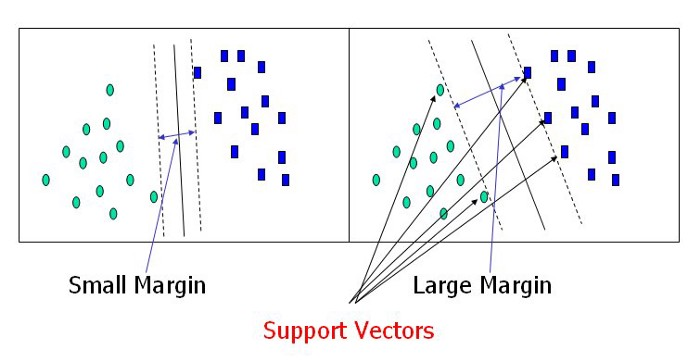
\includegraphics[scale=0.5]{svm}
	\caption{Ejemplo de SVM en dos dimensiones}
	\label{fig:svm}
\end{figure}
\section{XGBoost}
\label{alg:xgb}
Extreme Gradient Boosting es un método de aprendizaje combinado basado en árboles de decisión.\\
A diferencia de Random Forest (que también es un método combinado basado en árboles de decisión), XGBoost hace uso de técnicas de \textit{Gradient Boosting} frente a Random Forest que hace uso de \textit{Bagging} para entrenar los modelos que lo forman. (\ref{sec:rf}-\nameref{sec:rf}).\\
\linebreak
\textit{Boosting} se basa en la unión de varios modelos débiles para formar un modelo que en conjunto. Estos modelos débiles se van entrenando de forma iterativa, adaptando los parámetros del modelo en cada iteración, teniendo en cuenta que estos modelos no deben aumentar en complejidad y deben mantener un rendimiento mínimo (idealmente, mejor que un clasificador aleatorio).\\
\linebreak
\textit{Grandient Boosting} es un caso especial de \textit{Boosting} en el que se hace uso del algoritmo \textbf{Gradiente Descendente} para minimizar los errores de los modelos simples.\\
\linebreak
Finalmente, XGBoost funciona añadiendo secuencialmente Árboles de Decisión, de tal manera que cada árbol reduzca el error de los previos aprendiendo de los errores que han cometido los árboles anteriores.
\section{Perceptrón multi-capa}
\label{alg:mlp}
El Perceptrón Multicapa es un modelo de aprendizaje supervisado basada en red neuronales artificiales y haciendo uso del algoritmo \textbf{Perceptrón}.\\
\linebreak
El Perceptrón es un algoritmo de aprendizaje supervisado para clasificación binaria. Es un clasificador linear que funciona iterando sobre cada muestra del conjunto de datos hasta calcular un hiper-plano que separe el conjunto de datos. Los pasos de este algoritmo son:
\begin{enumerate}
	\item Establecer un plano inicial (generalmente de manera aleatoria ).
	\item Por cada muestra del conjunto de datos, si la muestra está mal clasificada, se modifican los pesos que definen el hiper-plano para clasificar correctamente esa muestra.
	\item El paso anterior se repite hasta que todas las muestras estén bien clasificadas ó no se haya hecho ninguna modificación. Por lo general, también se añade un número máximo de iteraciones que se van a realizar.
\end{enumerate}
Este algoritmo tiene una limitación muy fuerte: No puede resolver problemas no lineales (incluso funciones sencillas como la \textit{XOR}). \\
\linebreak
Para afrontar este problema, se propuso el usar una combinación de perceptrones siguiendo una estructura de red neuronal, consiguiendo así un modelo capaz de resolver problemas no lineales. Estas redes neuronales tienen al menos 3 capas:
\begin{itemize}
	\item Capa de entrada: Está formada por las primeras neuronas que forman la red y se encargan de introducir los datos a la red.
	\item Capa/s oculta: Son las capas de la zona media de la red y son las encargadas del procesamiento de los datos para formar el modelo.
	\item Capa de salida: Dan el valor de salida del modelo.
\end{itemize}
\begin{figure}[H]
	\centering
	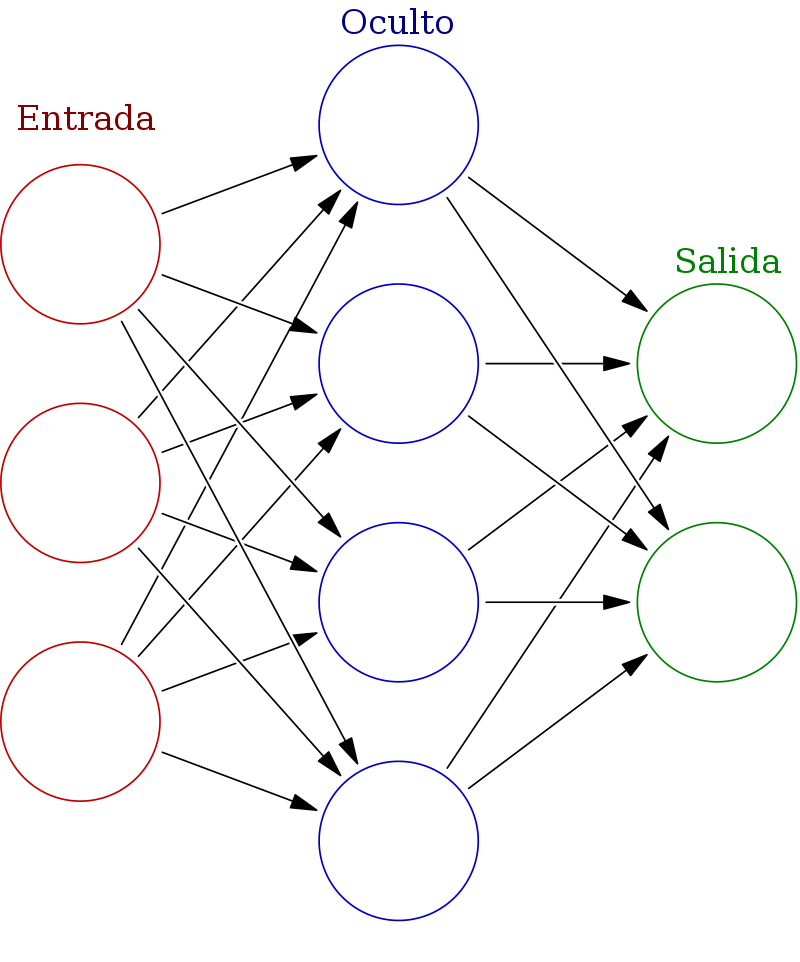
\includegraphics[scale=0.3]{rnn}
	\caption{Ejemplo de Red Neuronal con 1 capa oculta}
	\label{fig:rnn}
\end{figure}
Un elemento fundamental de las Redes Neuronales es el algoritmo de \textit{back-propagation}. Este algoritmo usa el error obtenido en las capas de salida y este era propagado hacia cada neurona anterior (de ahí el nombre de \textit{back-propagation}), ajustando así el peso calculado por cada neurona en función del comportamiento del modelo en la iteración anterior.


	\pagebreak

	\chapter{Regresión}
El objetivo principal de esta sección es el de comprobar el comportamiento de una serie de modelos e intentar mejorar el rendimiento de los mismos, añadiendo nuevos pasos a la etapa de pre-procesamiento y volviendo a entrenar los modelos que se han seleccionado. \\
Como se ha comentado previamente, se está trabajando sobre un problema bastante peculiar, donde se intenta predecir distintas variables ordinales. Antes de comenzar con algoritmos más complejos, el primer enfoque para resolver el problema ha sido el de usar una media de cada variable a predecir. \\
Es cierto que usando este enfoque, estamos perdiendo información muy importante: se está suponiendo que todas las variables son igualmente importantes, lo cual es una desventaja de esta aproximación al problema.
Por el contrario, este enfoque tiene la ventaja de estar usando algoritmos clásicos de regresión, proporcionando una salida más general, además de que usando este enfoque primero, descartamos la posibilidad de tener un conjunto de datos con mucho ruido o con un mal muestreo de los datos.
\section{Rendimiento de modelos de regresión}
Para comprobar el comportamiento de los distintos modelos seleccionados, se han usado las siguientes \textbf{métricas de regresión}: \textit{\textbf{Coeficiente de determinación}} (se denota como $R^2$), \textit{\textbf{Desviación de Poisson}} y \textit{\textbf{Error cuadrático medio}}
\subsection{Coeficiente de determinación}
Se define como \textbf{coeficiente de determinación} como la proporción de la varianza total explicada por la variables independientes del modelo. Proporciona una indicación de como de bueno es un ajuste y por tanto, una medida de como de bueno es el modelo cuando predice nuevas muestras.\\
\linebreak
Matemáticamente, se define el coeficiente de determinación como:
\[
	R^2 (y, \hat{y}) = 1 - \frac{\sum_{i=1}^{n}(y_i - \hat{y}_i)^2}    {\sum_{i=1}^{n} (y_i - \overline{y})^2}
\]

Donde:
\begin{itemize}
	\item $y$ es el conjunto de valores reales para las variables objetivo.
	\item $\hat{y}$ es el valor predicho para los valores objetivo.
	\item $\hat{y}_i$ es la predicción de la i-ésima muestra.
	\item $y_i$ es el valor real de la i-ésima muestra.
	\item $\overline{y} = \frac{1}{n} \sum_{i=1}^{n} y_i$.
	\item $n$ es el numero de muestras del conjunto.
\end{itemize}
insertar graficos explicando varianza, etc
\subsection{Desviación de Poisson}
\subsection{Error cuadrático medio}
El error cuadrático medio de un estimador mide el promedio de los errores al cuadrado.\\
Matemáticamente, se define el error cuadrático medio como:
\[
	MSE(y,\hat{y}) = \frac{1}{n} \sum_{i=1}^{n} (y_i - \hat{y}_i) ^2
\]
Donde:
\begin{itemize}
	\item $y$ es el conjunto de valores reales para las variables objetivo.
	\item $\hat{y}$ es el valor predicho para los valores objetivo.
	\item $\hat{y}_i$ es la predicción de la i-ésima muestra.
	\item $y_i$ es el valor real de la i-ésima muestra.
	\item $n$ es el numero de muestras del conjunto.
\end{itemize}

\subsection{Gráficos}
Además del uso de las métricas mencionadas previamente, se han creado las siguientes gráficas para visualizar los errores que esta haciendo un modelo en concreto. Esto ayuda a la toma de decisiones en fases siguientes.\\
Las gráficas que se han desarrollado son las siguientes:
\begin{itemize}
	\item Gráfico de dispersión de errores.
	\item Cantidad de errores por rango. (probablemente sea mejor cambiar este nombre, pero es el nombre que se me ocurrió)
\end{itemize}
El gráfico de dispersión de errores consiste en mostrar en la misma gráfica el valor real de las variables objetivo y el valor predicho por nuestro modelo. Esto nos permite ver como de juntos están las predicciones, identificando así en que zonas el algoritmo se está equivocando más frecuentemente.\\
\begin{figure}[H]
	\centering
	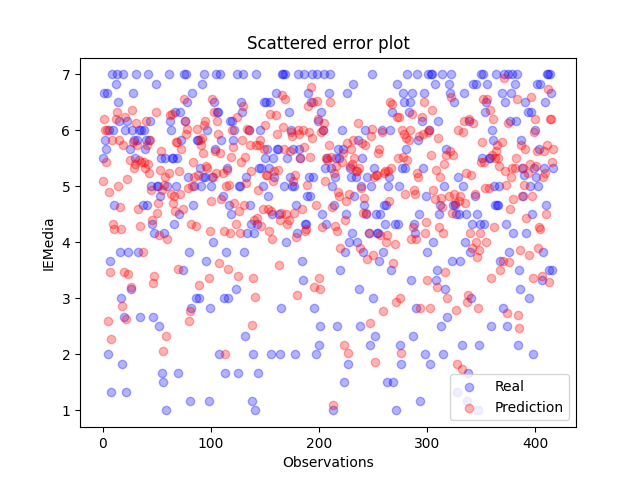
\includegraphics[scale=0.6]{scattered.png}
	\caption{Ejemplo de gráfico de dispersión de errores}
	\label{fig:scattered_example}
\end{figure}

El segundo gráfico consiste en lo siguiente:
Los modelos que han sido entrenados están prediciendo valores medios. El proceso seguido para realizar estos gráficos ha sido el de obtener los valores redondeados tanto de la predicción como del valor real. Si el valor redondeado de la predicción y del dato real son distintos, se ha considerado como error. Sumando estos errores, se puede generar un gráfico de barras como el siguiente para tener una visión más clara de en que zonas de la predicción el algoritmo esta funcionando peor:
\linebreak
\begin{figure}[H]
	\centering
	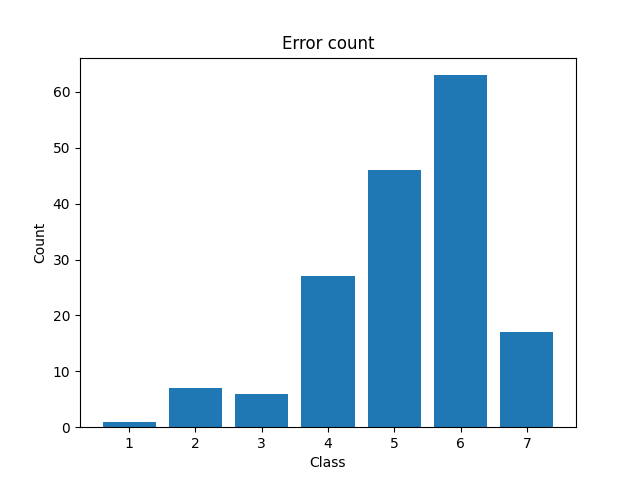
\includegraphics[scale=0.6]{error_hist.png}
	\caption{Ejemplo de gráfico de errores por rango}
	\label{fig:error_hist_example}
\end{figure}
\section{Modelos de regresión}
En esta sección, se va a mostrar los resultados obtenidos por los modelos seleccionados en \ref{sec:algoritmos}-\nameref{sec:algoritmos}.
\subsection{Árboles de decisión}
En esta sección se muestran los resultados obtenidos por el \textbf{Árboles de Decisión}, explicado en la sección \ref{alg:dec_tree}-\nameref{alg:dec_tree}.
\subsubsection*{Procesado de datos}
Antes de ejecutar la fase de entrenamiento, hay que modificar los datos para adaptarlos a las limitaciones del modelo. En este caso, los Árboles de Decisión no admiten valores perdidos y debido a ciertas limitaciones de la librería que se está usando, no son capaces de trabajar con variables categóricas, aunque generalmente si son capaces de trabajar con este tipo de variables..\\
Las modificaciones que se han hecho previamente son: (por orden)
\begin{enumerate}
	\item \textbf{Imputación de valores perdidos}
	\item \textbf{Transformación de variables categóricas a numéricas}
\end{enumerate}
Por este motivo, se ha tenido que introducir una fase extra transformando las variables categóricas en numéricas.
\subsubsection*{Resultados}
\label{sec:res_tree}
Antes de mostrar los resultados, hay que destacar que cuando se entrena un árbol de decisión sin limitar los parámetros, este va a seguir separando los datos de entrenamiento hasta que no pueda realizar más divisiones. Para encontrar el árbol óptimo, primero se ha entrenado el árbol por defecto y se han obtenido los parámetros. Esos parámetros se han establecido como limite, se han entrenado varios árboles con distintos parámetros (sin superar el límite establecido por el primer modelo) y se ha escogido el que mejores resultados obtenía. Los parámetros que mejor resultados dieron son: \\
\begin{itemize}
	\item \textbf{Profundidad máxima:} Limita la profundidad (cantidad de preguntas) del árbol. El mejor valor ha sido \textbf{8}
	\item \textbf{Máximo número de hojas:} Máximo numero de hojas (grupos en el último nivel de una rama). El mejor valor ha sido \textbf{16}
\end{itemize}
En esta sección se va a exponer los resultados obtenidos usando \textbf{Árboles de Decisión}.\\
La siguiente tabla expone los resultados obtenidos en validación:
\begin{table}[H]
	\centering
	\begin{tabular}{|c|c|c|c|c}
		\cline{1-4}
		FOLD   & R2    & Poisson Deviance & MSE   \\ \cline{1-4}
		Fold 0 & 0.678 & 0.211            & 0.886 \\ \cline{1-4}
		Fold 1 & 0.661 & 0.206            & 0.884 \\ \cline{1-4}
		Fold 2 & 0.629 & 0.239            & 0.98  \\ \cline{1-4}
		Fold 3 & 0.67  & 0.191            & 0.8   \\ \cline{1-4}
		Fold 4 & 0.636 & 0.211            & 0.933 \\ \cline{1-4}
		Fold 5 & 0.655 & 0.212            & 0.897 \\ \cline{1-4}
		Train  & 0.748 & 0.156            & 0.659 \\ \cline{1-4}
		Test   & 0.69  & 0.196            & 0.815 \\ \cline{1-4}
	\end{tabular}
	\caption{Árbol de decisión: Profundidad 8, número máximo de hojas 16}
	\label{tab:tree_res}
\end{table}
La siguiente figura muestra el gráfico de dispersión de errores:\\
\begin{figure}[H]
	\centering
	\includegraphics[scale=0.8]{src/scattered_error_DT.png}
	\caption{Gráfico de dispersión de errores}
	\label{fig:tree_scattered}
\end{figure}
Continuando con las gráficas, e continuación se muestra una gráfica con el conteo de errores por clase:
\begin{figure}[H]
	\centering
	\includegraphics[scale=0.8]{src/error_hist_DT.png}
	\caption{Conteo de errores}
	\label{fig:tree_error_plot}
\end{figure}
\subsubsection*{Representación}
Como se mencionó en la sección \textbf{\ref{alg:dec_tree}-\nameref{alg:dec_tree}}, los árboles de decisión tienen la ventaja de que pueden representarse fácilmente. \\
En este caso, vamos a usar una representación gráfica del árbol, las reglas que ha obtenido el árbol y las variables más importantes.\\
\linebreak
La siguiente figura muestra la representación gráfica del árbol de decisión entrenado:\\

\begin{figure}[H]
	\centering
	\includegraphics[scale=0.3]{src/dtree_plot.png}
	\caption{Árbol de decisión}
	\label{fig:decission_tree1}
\end{figure}
\pagebreak
Por ultimo, estas son las 10 variables que el modelo consideró con más relevancia. El valor asociado a cada variable es la \textbf{importancia Gini}:
\begin{figure}[H]
	\centering
	\includegraphics[scale=0.5]{src/feature_importance_DT}
	\caption{10 variables más importantes según Árboles de Decisión}
	\label{fig:feature_dtree}
\end{figure}
Volviendo a la documentación proporcionada para comprobar el significado de esos valores:
\begin{itemize}
	\item \textbf{AE5:} Pregunta 5 sobre Actitudes financieras empresariales. Valor $0.735667$
	\item \textbf{AcMedia:} Variable global de Actitud emprendedora. Valor $0.156046$
	\item \textbf{SE2:} Estoy preparado para iniciar una empresa viable. Valor $0.037300$
	\item \textbf{SE5:} Conozco cómo desarrollar un proyecto empresarial. Valor $0.014692$
	\item \textbf{NS1:} Mi familia aprobaría el que yo decidiese crear una empresa. Valor $0.012393$
	\item \textbf{Beca:} Tiene beca el encuestado. Valor $0.008256$
	\item \textbf{Nota:} Nota media del expediente académico hasta la fecha de la encuesta sobre 10 puntos. Valor $0.008034$
	\item \textbf{BA3.f:} En los últimos 12 meses, ¿has ahorrado personalmente algún dinero de alguna de las siguientes formas, independientemente de si aún dispones del dinero? Han contestado las opciones a, c, d, e, f, g (en casa, en cuenta de ahorro, darlo a la familia, productos de inversión, de otro modo). Valor $0.007389$
	\item \textbf{CEF19:} Pregunta sobre Conocimientos financieros empresariales. Valor $0.007202$
	\item \textbf{AE7:} Pregunta 7 sobre Actitudes financieras empresariales. Valor $0.006518$
\end{itemize}
De las columnas \textit{AEx} y \textit{CEFx} no hay información en la documentación, unicamente se menciona que son una serie de preguntas relacionadas con actitudes financieras empresariales y sobre conocimientos financieros empresariales respectivamente.
\subsection{Random Forest}
En esta sección se muestran los resultados obtenidos por el \textbf{Random Forest}, explicado en la sección \ref{alg:rf}-\nameref{alg:rf}.
\subsubsection*{Procesado de datos}
Al igual que los árboles de decisión, se ha hecho una imputación de valores perdidos y se ha transformado las variables categóricas a numéricas debido a limitación que hay en la librería usada.
\pagebreak
\subsubsection*{Resultados}
Antes de mostrar los resultados, estos son los parámetros que se han usado al entrenar el modelo:
\begin{itemize}
	\item \textbf{max\_features}: Número de variables que se van a escoger de manera aleatoria: $\frac{1}{3}$ del número de variables.
	\item\textbf{n\_estimators}: Número de árboles que forman el Random Forest: $500$
\end{itemize}
En la siguiente tabla, se muestra el resultado para obtenidos en validación y en test:
\linebreak
\begin{table}[H]
	\centering
	\begin{tabular}{|c|c|c|c|c}
		\cline{1-4}
		FOLD   & R2    & Poisson Deviance & MSE   \\ \cline{1-4}
		Fold 0 & 0.767 & 0.155            & 0.642 \\ \cline{1-4}
		Fold 1 & 0.775 & 0.137            & 0.586 \\ \cline{1-4}
		Fold 2 & 0.741 & 0.17             & 0.684 \\ \cline{1-4}
		Fold 3 & 0.736 & 0.151            & 0.64  \\ \cline{1-4}
		Fold 4 & 0.747 & 0.15             & 0.649 \\ \cline{1-4}
		Fold 5 & 0.753 & 0.153            & 0.64  \\ \cline{1-4}
		Train  & 0.967 & 0.023            & 0.087 \\ \cline{1-4}
		Test   & 0.769 & 0.149            & 0.606 \\ \cline{1-4}
	\end{tabular}
	\caption{Random Forest}
	\label{tab:res_random_forest}
\end{table}
La siguiente figura muestra el gráfico de dispersión de errores:\\
\linebreak
\begin{figure}[H]
	\centering
	\includegraphics[scale=0.7]{src/scattered_error_rf.png}
	\caption{Gráfico de dispersión de errores}
	\label{fig:rf_scattered}
\end{figure}
Continuando con las gráficas, e continuación se muestra una gráfica con el conteo de errores por clase:
\begin{figure}[H]
	\centering
	\includegraphics[scale=0.7]{src/error_hist_rf.png}
	\caption{Conteo de errores}
	\label{fig:rf_error_plot}
\end{figure}
Para finalizar, esta es la lista de las 10 variables más importantes que ha obtenido Random Forest:
\begin{figure}[H]
	\centering
	\includegraphics[scale=0.6]{src/feature_importance_rf}
	\caption{10 variables más importantes según Random Forest}
	\label{fig:feature_rf}
\end{figure}
Volviendo a la documentación, esta es la explicación para cada variable:
\begin{itemize}
	\item\textbf{AE5:} Pregunta 5 sobre Actitudes financieras empresariales. Valor = $0.246364$
	\item\textbf{AcMedia:} Variable global de Actitud emprendedora. Valor = $0.220202$
	\item\textbf{AC2:} Ser emprendedor es una salida profesional atractiva para mí. Valor = $0.072907$
	\item\textbf{AC4:}Ser emprendedor supondría una gran satisfacción para mí. Valor = $0.065776$
	\item\textbf{AC3:} Si tuviera la oportunidad y los recursos, me gustaría iniciar una empresa. Valor = $0.041642$
	\item\textbf{SEMedia:} Variable global de Autoeficacia emprendedora. Valor = $0.022872$
	\item\textbf{SE2:} Estoy preparado para iniciar una empresa viable. Valor = $0.019630$
	\item\textbf{AC1:} Ser emprendedor implica más ventajas que desventajas para mí. Valor = $0.019396$
	\item\textbf{NS1:} Mi familia aprobaría el que yo decidiese crear una empresa. Valor = $0.014467$
	\item\textbf{Nota:} Nota media del expediente académico hasta la fecha de la encuesta sobre 10 puntos. Valor = $0.012254$
\end{itemize}
\subsection{KNN}
En esta sección se muestran los resultados obtenidos por el \textbf{K-Nearest Neighbor}, explicado en la sección \ref{alg:knn}-\nameref{alg:knn}.
\subsubsection*{Procesado de datos}
KNN es un algoritmo que depende de la distancia entre dos muestras, esto implica que si una caracteristica del conjunto de datos que se esta usando tiene un rango \textbf{mayor} que otra, esa característica aportará más al cálculo de la distancia, cuando no necesariamente debe de ser así. Por ese motivo, este algoritmo necesita que el conjunto de datos esté \textbf{normalizado} en el momento de entrenar.\\
\linebreak
Este algoritmo, a parte de necesitar que los datos estén normalizados, no admite valores perdidos y variables categóricas.

\subsubsection*{Resultados}
Antes de mostrar los resultados, estos son los parámetros que se han usado al entrenar el algoritmo:
\begin{itemize}
	\item \textbf{K:} Número de vecinos: 5
	\item \textbf{Métrica:} Distancia usada: Minkowski con $P=2$ (distancia euclidiana).
\end{itemize}
En la siguiente tabla, se muestra el resultado para obtenidos en validación y en test:
\linebreak
\begin{table}[H]
	\centering
	\begin{tabular}{|c|c|c|c|c}
		\cline{1-4}
		FOLD   & R2    & Poisson Deviance & MSE   \\ \cline{1-4}
		Fold 0 & 0.47  & 0.356            & 1.46  \\  \cline{1-4}
		Fold 1 & 0.407 & 0.378            & 1.545 \\  \cline{1-4}
		Fold 2 & 0.449 & 0.362            & 1.457 \\  \cline{1-4}
		Fold 3 & 0.435 & 0.329            & 1.372 \\  \cline{1-4}
		Fold 4 & 0.467 & 0.321            & 1.367 \\  \cline{1-4}
		Fold 5 & 0.446 & 0.349            & 1.44  \\  \cline{1-4}
		Train  & 0.653 & 0.227            & 0.907 \\ \cline{1-4}
		Test   & 0.527 & 0.301            & 1.242 \\ \cline{1-4}
	\end{tabular}
	\caption{KNN: $K=5$, métrica Minkowski con $P=2$}
	\label{tab:knn_res}
\end{table}
La siguiente figura muestra el gráfico de dispersión de errores:
\begin{figure}[H]
	\centering
	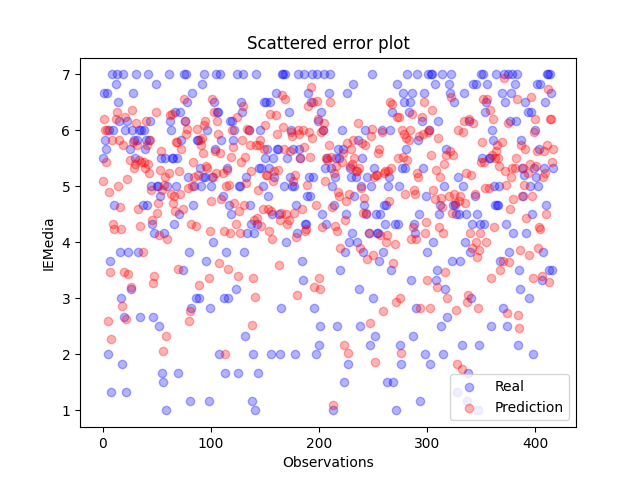
\includegraphics[scale=0.8]{src/scattered_error_knn.png}
	\caption{Gráfico de dispersión de errores}
	\label{fig:knn_scattered}
\end{figure}
Continuando con las gráficas, e continuación se muestra una gráfica con el conteo de errores por clase:\\
\linebreak
\begin{figure}[H]
	\centering
	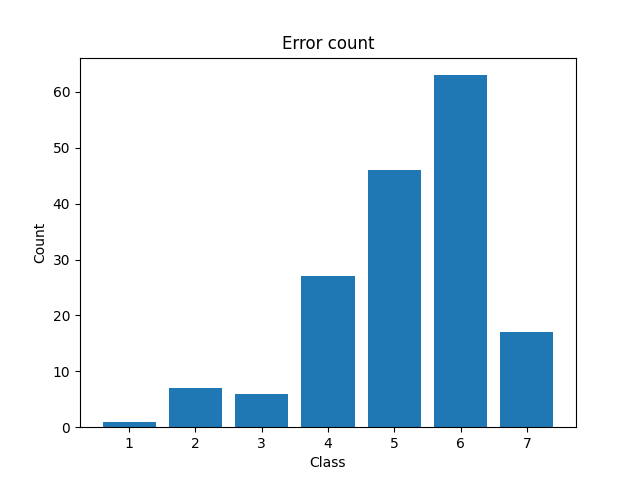
\includegraphics[scale=0.8]{src/error_hist_knn.png}
	\caption{Conteo de errores}
	\label{fig:knn_error_plot}
\end{figure}
\subsection{SVM}
En esta sección se muestran los resultados obtenidos por el \textbf{Support Vector Machines}, explicado en la sección \ref{alg:svm}-\nameref{alg:svm}.
\subsubsection*{Procesado de datos}
SVM son modelos con una fuerte base matemática, por lo que son modelos que no pueden ser entrenados usando variables categóricas.
Las modificaciones que se han hecho previamente son: (por orden)
\begin{enumerate}
	\item \textbf{Imputación de valores perdidos.}
	\item \textbf{Escalado de valores numéricos.}
	\item \textbf{Transformación de variables categóricas a numéricas.}
\end{enumerate}
\subsubsection*{Resultados}
A continuación se muestra una tabla con los resultados obtenidos por SVM en el conjunto de validación y en el conjunto de test:
\begin{table}[H]
	\centering
	\begin{tabular}{|c|c|c|c|c}
		\cline{1-4}
		FOLD   & R2    & Poisson Deviance & MSE   \\ \cline{1-4}
		Fold 0 & 0.671 & 0.236            & 0.906 \\ \cline{1-4}
		Fold 1 & 0.718 & 0.186            & 0.734 \\ \cline{1-4}
		Fold 2 & 0.728 & 0.185            & 0.72  \\ \cline{1-4}
		Fold 3 & 0.691 & 0.192            & 0.75  \\ \cline{1-4}
		Fold 4 & 0.697 & 0.193            & 0.776 \\ \cline{1-4}
		Fold 5 & 0.701 & 0.198            & 0.777 \\ \cline{1-4}
		Train  & 0.894 & 0.076            & 0.276 \\ \cline{1-4}
		Test   & 0.737 & 0.173            & 0.691 \\ \cline{1-4}
	\end{tabular}
	\caption{SVM: Tolerancia $1^{-3}$, Kernel RBF, $C=1$}
	\label{tab:svm_res}
\end{table}
La siguiente figura muestra el gráfico de dispersión de errores:
\begin{figure}[H]
	\centering
	\includegraphics[scale=0.8]{src/scattered_error_svr.png}
	\caption{Gráfico de dispersión de errores}
	\label{fig:svr_scattered}
\end{figure}
Continuando con las gráficas, e continuación se muestra una gráfica con el conteo de errores por clase:\\
\linebreak
\begin{figure}[H]
	\centering
	\includegraphics[scale=0.8]{src/error_hist_svr.png}
	\caption{Conteo de errores}
	\label{fig:svr_error_plot}
\end{figure}
\subsection{XGBoost}
En esta sección se muestran los resultados obtenidos por el \textbf{Xtreme Gradient Boosting}, explicado en la sección \ref{alg:xgb}-\nameref{alg:xgb}.
\subsubsection*{Procesado de datos}
El pre-procesado aplicado para este modelo ha sido similar al usado en Árboles de Decisión:
\begin{enumerate}
	\item \textbf{Imputación de valores perdidos}
	\item \textbf{Transformación de variables categóricas a numéricas}
\end{enumerate}
\subsubsection*{Resultados}
A continuación se muestra una tabla con los resultados obtenidos por \textbf{XGBoost} en los conjuntos de validación, train y test:
\begin{table}[H]
	\centering
	\begin{tabular}{|c|c|c|c|c|}
		\cline{1-4}
		FOLD   & R2    & Poisson Deviance & MSE   \\ \cline{1-4}
		Fold 0 & 0.726 & 0.186            & 0.754 \\ \cline{1-4}
		Fold 1 & 0.734 & 0.165            & 0.693 \\ \cline{1-4}
		Fold 2 & 0.71  & 0.196            & 0.766 \\ \cline{1-4}
		Fold 3 & 0.723 & 0.16             & 0.671 \\ \cline{1-4}
		Fold 4 & 0.744 & 0.157            & 0.658 \\ \cline{1-4}
		Fold 5 & 0.727 & 0.173            & 0.708 \\ \cline{1-4}
		Train  & 0.991 & 0.005            & 0.024 \\ \cline{1-4}
		Test   & 0.741 & 0.162            & 0.68  \\ \cline{1-4}
	\end{tabular}
	\caption{Métricas de XGBoost con}
	\label{tab:xgboost}
\end{table}
La siguiente figura muestra el gráfico de dispersión de errores:
\begin{figure}[H]
	\centering
	\includegraphics[scale=0.8]{src/scattered_error_xgboost.png}
	\caption{Gráfico de dispersión de errores para XGBoost}
	\label{fig:xgboost_scattered}
\end{figure}
Finalizando con las gráficas, a continuación se muestra una gráfica con el conteo de errores por clase:
\begin{figure}[H]
	\centering
	\includegraphics[scale=0.8]{src/error_hist_xgboost.png}
	\caption{Conteo de errores}
	\label{fig:xgboost_error_plot}
\end{figure}
\subsection{Perceptrón multi-capa}
En esta sección se muestran los resultados obtenidos por el \textbf{Perceptron multicapa}, explicado en la sección \ref{alg:mlp}-\nameref{alg:mlp}.
\subsubsection*{Procesado de datos}
MLP es un algoritmo que no es capaz de ser entrenados usando variables categóricas. Las modificaciones que se han hecho sobre el conjunto de datos son las siguientes:
\begin{enumerate}
	\item \textbf{Imputación de valores perdidos.}
	\item \textbf{Escalado de valores numéricos.}
	\item \textbf{Transformación de variables categóricas a numéricas.}
\end{enumerate}
\subsubsection*{Resultados}
En esta sección se va a mostrar los resultados obtenidos por el Perceptrón Multi-capa. \\
\linebreak
En esta tabla, se puede observar el rendimiento del modelo en los conjuntos de validación, entrenamiento y test:
\begin{table}[H]
	\centering
	\begin{tabular}{|c|c|c|c|c}
		\cline{1-4}
		FOLD   & R2    & Poisson Deviance & MSE   \\\cline{1-4}
		Fold 0 & 0.557 & 0.321            & 1.221 \\\cline{1-4}
		Fold 1 & 0.566 & 0.274            & 1.13  \\\cline{1-4}
		Fold 2 & 0.586 & 0.269            & 1.096 \\\cline{1-4}
		Fold 3 & 0.412 & 0.291            & 1.427 \\\cline{1-4}
		Fold 4 & 0.488 & 0.303            & 1.313 \\\cline{1-4}
		Fold 5 & 0.522 & 0.292            & 1.237 \\\cline{1-4}
		Train  & 0.999 & 0.0              & 0.002 \\\cline{1-4}
		Test   & 0.616 & 0.27             & 1.007 \\\cline{1-4}
	\end{tabular}
	\caption{Perceptrón Multicapa: 1 capa oculta con 100 neuronas, 500 iteraciones max}
	\label{tab:mlp_res}
\end{table}
La siguiente figura muestra el gráfico de dispersión de errores:
\begin{figure}[H]
	\centering
	\includegraphics[scale=0.8]{src/scattered_error_MLP.png}
	\caption{Gráfico de dispersión de errores}
	\label{fig:mlp_scattered}
\end{figure}
Continuando con las gráficas, e continuación se muestra una gráfica con el conteo de errores por clase:\\
\linebreak
\begin{figure}[H]
	\centering	\includegraphics[scale=0.8]{src/error_hist_MLP.png}
	\caption{Conteo de errores}
	\label{fig:mlp_error_plot}
\end{figure}
\section{Análisis de resultados}
Se ha observado que los modelos basados en Árboles de Decisión y Random Forest han tenido un buen comportamiento, por lo que se ha optado por seguir haciendo uso de ellos en secciones siguientes. XGBoost, tiene unos resultados ligeramente peores respecto a Random Forest pero con un comportamiento similar, fallando considerable en valores altos de intención emprendedora media). Como XGBoost no esta aportando nada nuevo, por ahora se va a descartar.\\
\linebreak
SVR se ha comportado casi al nivel de modelos como XGBoost o Random Forest. Por ahora, no se va a descartar su uso, ya que introduciendo el conocimiento que se ha obtenido usando modelos como Random Forest o árboles de decisión se podría mejorar el rendimiento.\\
\linebreak
Los resultados obtenidos por  KNN demuestran que este algoritmo no funciona bien con el conjunto de datos que se está usando. La razón más probable por la que KNN obtuvo estos resultados, es que hay relaciones entre las variables que KNN no es capaz de detectar, al comparar únicamente la distancia característica por característica. Debido al bajo desempeño que se ha obtenido al usar KNN, va a ser descartado de las siguientes fases.\\
\linebreak
Respecto al Perceptrón Multicapa, ya que el rendimiento en comparación con otros modelos probados y debido al enorme coste de entrenamiento que pueden llegar a tener, se ha decidido no continuar haciendo uso de este modelo.\\
\linebreak
Como ya se ha mencionado, los modelos basados en árboles de decisión son capaces de obtener la importancia de las características. A continuación se muestran las gráficas de nuevo para facilitar la comparación:
\begin{figure}[H]
	\centering
	\includegraphics[scale=0.5]{src/feature_importance_DT}
	\caption{10 variables más importantes según árboles de decisión}
	\label{fig:feature_dtree2}
\end{figure}
\begin{figure}[H]
	\centering
	\includegraphics[scale=0.5]{src/feature_importance_rf}
	\caption{10 variables más importantes según RF}
	\label{fig:feature_rf2}
\end{figure}
Como se ve en las figuras, vemos que hay dos variables que \textbf{ambos} algoritmos han dado como más importantes:
\begin{itemize}
	\item\textbf{AE5:} Pregunta  5 sobre Actitudes financieras empresariales.
	\item\textbf{AcMedia:} Variable global de Actitud emprendedora.
\end{itemize}
Repasando los resultados, se puede apreciar que a todos los algoritmos usados les está costando predecir correctamente los valores altos para la intención emprendedora media (véase figura \ref{fig:rf_error_plot}). Este comportamiento ha sido constante para cada algoritmo usado. La causa de este comportamiento puede ser que a medida que se incrementa el valor de intención emprendedora media, los datos son menos dispersos y a los algoritmos les está costando distinguir entre varios valores cercanos. Este comportamiento se puede apreciar en los gráficos de dispersión de errores que se han mostrado previamente.
\pagebreak
\section{Muestreo de datos}
Una vez se ha comprobado el rendimiento de los distintos modelos que se han seleccionado, se va a intentar mejorarlo añadiendo nuevas etapas extra al procesamiento de datos antes de entrenar los modelos.
\newline
Como se ha podido observar en la primera iteración, todos los algoritmos se están equivocando en valores altos. Para intentar reducir el ruido, se va tratar el conjunto de datos haciendo \textbf{under-sampling}.\\
Under-Sampling (se podría traducir como \textit{muestreo}) es una técnica para reducir el ruido del conjunto de datos eliminando algunas muestras del conjunto de datos.\\
\linebreak
Como se puede ver en la \ref{tab:ocurrencia_valores} donde se muestra la ocurrencia de valores para las distintas variables a predecir,  aquellos con un valor alto son los más predominantes, siendo en estos valores donde los algoritmos más se están equivocando. El motivo puede ser que al estar prediciendo la media de las distintas variables, se está introduciendo una gran cantidad de ruido. \\
En valores bajos, como se puede ver en la figura \ref{fig:rf_error_plot} donde se muestra el gráfico de errores para Random Forest, la cantidad de fallos en el algoritmo para estos valores es mucho menor. Esta tendencia se repite en todos los algoritmos.\\
\subsection{Algoritmo}
Para realizar el proceso de muestreo, se ha desarrollado el siguiente algoritmo:
\begin{enumerate}
	\item Se entrena un modelo de aprendizaje con el conjunto de entrenamiento.
	\item Por cada muestra del conjunto de entrenamiento, se predice el valor usando el modelo entrenado.
	\item Se comprueba la diferencia entre valor real y el valor predicho.
	\item Si la diferencia es mayor que un umbral, se elimina esa muestra del conjunto de entrenamiento.
\end{enumerate}
La función que ejecuta este simple algoritmo de muestreo se llama \textit{\textbf{regression\_under\_sampler}}.
\linebreak
El modelo entrenado para hacer muestreo, es un árbol de decisión con un máximo de $4$ niveles, eliminando muestras de todo el rango de predicción.
\subsection{Resultados}
A continuación se muestra una serie de gráficos comparando los resultados obtenidos por los algoritmos seleccionados:
\subsubsection*{Árboles de Decisión}
\begin{figure}[H]
	\centering
	\includegraphics[scale=0.8]{src/dtree_undersamp_error_hist.png }
	\caption{Comparación de errores usando under-sampling}
	\label{fig:cmp_error_dtree}
\end{figure}
Como se aprecia en la figura \ref{fig:cmp_error_dtree}, usando el algoritmo de muestreo, se ha reducido la cantidad ruido en los rangos más altos de predicción, mejorando así el rendimiento del árbol de decisión para estos valores y estabilizando las zonas donde se estaba comportando peor.
\begin{figure}[H]
	\centering
	\includegraphics[scale=0.8]{src/dtree_undersamp_val_metrics.png}
	\caption{Media en validación usando under-sampling}
	\label{fig:cmp_val_dtree}
\end{figure}
Esta gráfica compara el rendimiento medio en el conjunto de validación.
Respecto a las métricas obtenidas en los conjuntos de validación, se puede apreciar que en cuanto al valor obtenido por $R2$ se ha mantenido, pero se ha mejorado drásticamente el valor en las métricas \textit{Desviación de Poisson} y \textit{MSE}. Esto indica que el modelo obtenido tras el procesamiento se ajusta mejor a los datos.
\begin{figure}[H]
	\centering
	\includegraphics[scale=0.8]{src/dtree_undersamp_test_metrics.png}
	\caption{Métricas en test usando under-sampling}
	\label{fig:cmp_test_dtree}
\end{figure}
Como se puede ver en la imagen anterior, las métricas en test son ligeramente mejores tras reducir el ruido dentro del conjunto de entrenamiento.\\
\linebreak
En general, se aprecia una mejora en árboles de decisión reduciendo el ruido del conjunto de datos, ya que los árboles de decisión son algoritmos bastantes sensibles al ruido.
\subsubsection*{SVR}
\begin{figure}[H]
	\centering
	\includegraphics[scale=0.8]{src/svr_undersamp_error_hist.png }
	\caption{Comparación de errores usando under-sampling}
	\label{fig:cmp_error_svr}
\end{figure}
Al contrario que los Árboles de Decisión, SVM han sido menos propicias al ruido del conjunto de datos. Al aplicar el muestreo se aprecia una bajada de rendimiento en todos los rangos de predicción. \\
Como se explicaba en \nameref{sec:svm} - \ref{sec:svm}, SVM busca el hiperplano con más margen entre los clusters que forma el conjunto de datos, consiguiendo así un algoritmo robusto frente a ruido.
\begin{figure}[H]
	\centering
	\includegraphics[scale=0.8]{src/svr_undersamp_val_metrics.png}
	\caption{Media en validación usando under-sampling}
	\label{fig:cmp_val_svr}
\end{figure}
\begin{figure}[H]
	\centering
	\includegraphics[scale=0.8]{src/svr_undersamp_test_metrics.png}
	\caption{Métricas en test usando under-sampling}
	\label{fig:cmp_test_svr}
\end{figure}
Las gráficas \ref{fig:cmp_val_svr} y \ref{fig:cmp_test_svr} complementan el resultado mostrado en la gráfica \ref{fig:cmp_error_svr}, las cuales demuestran que la mejora apreciada en Árboles de Decisión no ha aplicó en SVM y lejos de mejorar, ha empeorado el valor obtenido por algunas métricas de regresión.\\
\subsubsection*{Random Forest}
\begin{figure}[H]
	\centering
	\includegraphics[scale=0.8]{src/rf_undersamp_error_hist.png }
	\caption{Comparación de errores usando under-sampling}
	\label{fig:cmp_error_rf}
\end{figure}
En la figura se puede apreciar como al igual que los Árboles de decisión, el eliminar ciertas instancias ruidosas del conjunto de datos implica una mejora en el rendimiento del algoritmo. En este caso, se ha conseguido reducir el porcentaje de fallos cuando se está prediciendo valores altos de intención emprendedora media.
\begin{figure}[H]
	\centering
	\includegraphics[scale=0.8]{src/rf_undersamp_val_metrics.png}
	\caption{Media en validación usando under-sampling}
	\label{fig:cmp_val_rf}
\end{figure}
En cuanto a la media en validación, a medida que se reduce la cantidad de muestras eliminadas, se aprecia como se reduce la métrica $R2$ pero mejora las métricas MSE y Desviación Poisson.
\begin{figure}[H]
	\centering
	\includegraphics[scale=0.8]{src/rf_undersamp_test_metrics.png}
	\caption{Métricas en test usando under-sampling}
	\label{fig:cmp_test_rf}
\end{figure}
En test se aprecia el mismo comportamiento que en los conjuntos de validación: el mejor valor para $R2$ ha sido el obtenido entrando el modelo sin aplicar el  muestreo, mientras que respecto al resto de métricas, ha obtenido los mejores resultados eliminando las muestras problemáticas.\\
\subsection{Análisis de resultados}
Se ha apreciado una mejora en en los algoritmos basados en árboles de decisión. La principal mejora ha sido el obtener una menor cantidad de errores en aquellas zonas donde los algoritmos se están comportando peor. También se ha podido observar que Random Forest obtuvo mejores resultados con un umbral más alto que Árboles de Decisión. \\
La causa más probable de que necesite un umbral más alto es que al usar varios árboles para predecir el resultado, la probabilidad de que varios árboles contradigan el valor predicho por un árbol que clasificó mal un valor es alta. Por eso, al eliminar aquellas muestras más problemáticas del conjunto, el propio Random Forest es capaz de lidiar con el ruido de muestras que son menos problemáticas y beneficiarse de tener un conjunto de entrenamiento más grande.\\
\linebreak
Respecto a SVM, observando los resultados obtenidos, se aprecia que ha medida que se reduce la cantidad de muestras que se eliminan, el rendimiento es mejor.
Como se están eliminando muestras que pueden estar en la frontera (o incluso vectores soporte),, es posible que el hiper-plano calculado por el modelo de un menor margen o sea en general peor.

	\pagebreak

	\chapter{Clasificación}
\label{sec:class}
Se ha comprobado que usando regresión, se ha conseguido unos buenos resultados a la hora de predecir un valor \textbf{preciso} de la intención emprendedora media. El siguiente paso realizado ha sido el de \textbf{categorizar} el caso de regresión, obteniendo así clases del tipo \textit{intención emprendedora alta, baja o media}.\\
Hay que recordar que el resultado obtenido por el modelo de aprendizaje puede ser leído por personal no familiarizado con matemáticas o informática. Este enfoque lo que nos permite es usar una única variable como objetivo con los valores \textit{alto, bajo o alto}, siendo así más legible la salida del algoritmo.\\
\linebreak
Para categorizar los valores de predicción se ha establecido unos rangos y se van a transformar los valores de ese rango en las clases alta. media. y baja. Para establecer el rango, se ha ejecutado varias veces los algoritmos seleccionados y se han comparado las métricas obtenidas, usando unos rangos para establecer estas clases.\\
Los rangos que se han probado son:
\begin{itemize}
	\item $(4, 6, 7)$
	\item $(3.5, 5.5, 7)$
	\item $(3, 5, 7)$
\end{itemize}
Estas tuplas representan el valor usado para determinar el valor límite para clasificar una muestra como emprendimiento bajo, medio o alto (en ese orden).\\
\linebreak
Al igual que en regresión (\ref{sec:validation}-\nameref{sec:validation}), se ha usado la técnica de \textit{k-fold validation} para validar el rendimiento de los modelos entrenados.
\clearpage
\section{Modelos de clasificación}
Para clasificación, se van a usar unicamente aquellos modelos que se ha demostrado empíricamente en la sección \ref{sec:algoritmos}-\nameref{sec:algoritmos} que han tenido un buen desempeño. Por tanto se van a usar Árboles de Decisión, Random Forest y SVM.
\section{Métricas usadas}
Para validar el rendimiento de los modelos seleccionados se van a usar las siguientes métricas:
\begin{itemize}
	 \item \textbf{Métrica F1}
	 \item \textbf{Área bajo la curva (AUC)}
	 \item \textbf{Precisión}
\end{itemize}
Se puede encontrar una explicación más exhaustiva de estas métricas en la Sección \ref{metric:class}.\\
\linebreak
En las secciones siguientes se podrá encontrar los resultados de estas métricas para los distintos modelos que se han seleccionado. Finalmente, se valorará si este enfoque es correcto o no, junto con posibles mejoras y correcciones.\\
\linebreak
Los resultados obtenidos se van a mostrar usando gráficas representando los valores obtenidos para las distintas métricas que se están usando. Además de estas gráficas, también se mostrarán las Matrices de Confusión obtenidas por los modelos usando los distintos conjuntos de datos que se han obtenido usando este enfoque, y, finalmente, se mostrará una tabla con los resultados numéricos de las métricas obtenidas.e
\clearpage
\subsection{Árboles de Decisión}
\label{class:dt1}
En esta sección se va a exponer los resultados obtenidos en clasificación usando \textbf{Árboles de Decisión}.\\
Se va a comenzar mostrando los valores de las 3 métricas seleccionadas para los conjuntos de validación en los 3 conjuntos de datos obtenidos:
\begin{figure}[H]
	\centering
	\includegraphics[scale=0.7]{src/dt_cmp_val_metrics}
	\caption{Comparación en conjunto de validación}
	\label{fig:dtre_class_val}
\end{figure}
Se puede observar como aún eliminando cierta información del conjunto, ese conocimiento no se ha perdido, ya que se puede observar que en los conjuntos de validación se han obtenido unas valores muy buenos para los 3 conjuntos. \\
\linebreak
Se puede observar como parece que al usar los conjuntos $(3,5,7)$ y $(3.5,5.5,7)$ no existe una diferencia observable, ya que los valores de todas las métricas es el mismo. \\
El único conjunto que parece que cambia de comportamiento es el $(4,6,7)$, donde se observa una ligera mejora en la métrica F1, una mínima reducción del AUC y una bajada en el accuracy. Hay que tener en cuenta que se está mostrando la \textbf{media} de las métricas calculadas en cada \textit{fold} de la validación cruzada. Puede ocurrir que en uno de los conjuntos, se haya obtenido un conjunto para el que el modelo ha rendido peor.
\clearpage
\begin{figure}[H]
	\centering
	\includegraphics[scale=0.7]{src/dt_cmp_test_metrics}
	\caption{Comparación en conjunto de test}
	\label{fig:dtre_class_testl}
\end{figure}
Se puede observar que se han repetido \textbf{algunos} de los comportamientos observados en la validación: para los conjunto $(3,5,7)$ y $(3.5,5.5,7)$ no existe una diferencia observable en el valor de las medias calculadas. \\
A diferencia que en validación, en test el modelo entrenado con el conjunto $(4,6,7)$ se ha comportado ligeramente mejor. Una hipótesis para explicar este comportamiento podría ser que al dar más margen para valores bajos e intermedios, estos valores disponen de más instancias y el modelo ha sido capaz de aprovecharlo.\\
\linebreak
Al observar que los conjuntos $(3,5,7)$ y $(3.5,5.5,7)$ no presentan diferencias observables, se va a descartar el modelo entrenado con uno de los conjuntos, ya que no esta aportando valor.\\
\linebreak
Para ampliar estos resultados, a continuación se va a mostrar unas tablas con los valores de las métricas obtenidas por cada conjunto.
\subsubsection*{Tablas de métricas}
\begin{table}[H]
	\centering
	\begin{tabular}{|c|c|c|c|c}
		\cline{1-4}
		FOLD   & F1 Score & AUC Score & Accuracy \\ \cline{1-4}
		Fold 0 & 0.684    & 0.822     & 0.713    \\ \cline{1-4}
		Fold 1 & 0.699    & 0.881     & 0.725    \\ \cline{1-4}
		Fold 2 & 0.691    & 0.84      & 0.713    \\ \cline{1-4}
		Fold 3 & 0.664    & 0.833     & 0.701    \\ \cline{1-4}
		Fold 4 & 0.753    & 0.869     & 0.768    \\ \cline{1-4}
		Fold 5 & 0.698    & 0.849     & 0.724    \\ \cline{1-4}
		Train  & 0.781    & 0.909     & 0.794    \\ \cline{1-4}
		Test   & 0.701    & 0.843     & 0.715    \\ \cline{1-4}
	\end{tabular}
	\caption{Valores de métricas obtenidos usando rango $(3.5,5.5,7)$}
\end{table}
\begin{table}[H]
	\centering
	\begin{tabular}{|c|c|c|c|c}
		\cline{1-4}
		FOLD   & F1 Score & AUC Score & Accuracy \\ \cline{1-4}
		Fold 0 & 0.709    & 0.861     & 0.705    \\ \cline{1-4}
		Fold 1 & 0.686    & 0.828     & 0.681    \\ \cline{1-4}
		Fold 2 & 0.698    & 0.842     & 0.697    \\ \cline{1-4}
		Fold 3 & 0.715    & 0.855     & 0.709    \\ \cline{1-4}
		Fold 4 & 0.69     & 0.836     & 0.688    \\ \cline{1-4}
		Fold 5 & 0.7      & 0.844     & 0.696    \\ \cline{1-4}
		Train  & 0.752    & 0.89      & 0.746    \\ \cline{1-4}
		Test   & 0.721    & 0.867     & 0.72     \\ \cline{1-4}
	\end{tabular}
	\caption{Valores de métricas obtenidos usando rango $(4,6,7)$}
\end{table}
Por lo general, se han obtenido unos muy buenos resultados usando ambos rangos, extrayendo un conocimiento importante.
\clearpage
A continuación, las tablas con los resultados de las métricas y las matrices de confusión obtenidas por los Árboles de decisión usando la categorización usando los rangos $(3.5,5.5,7)$ y $(4,6,7)$
\subsubsection*{Matrices de confusión}
\begin{figure}[H]
	\centering
	\includegraphics[scale=0.5]{src/confusion_matrix_dtree_classification_3-5_5-5_7.png}
	\caption{Matriz de confusión para Árboles de Decisión usando $(3.5,5.5,7)$}
	\label{fig:confusion_matrix_dtree1}
\end{figure}
Se puede observar en la Figura \ref{fig:confusion_matrix_dtree1} como el modelo ha tenido complicaciones a la hora de predecir valores bajos, confundiendo más de la mitad de estos valores con valores que realmente son valores medios.\\
En valores medios y valores altos, el rendimiento ha sido muy bueno, clasificando correctamente una buena porción de las muestras.
\clearpage
\begin{figure}[H]
	\centering
	\includegraphics[scale=0.5]{src/confusion_matrix_dtree_classification_4_6_7}
	\caption{Matriz de confusión para Árboles de Decisión usando $(4,6,7)$}
	\label{fig:confusion_matrix_dtree2}
\end{figure}
A diferencia del modelo entrenado con el anterior conjunto, con este se puede observar una mejora en los valores bajos y se mantiene la cantidad de valores medios y altos que se han predicho correctamente en el anterior modelo.\\
Tiene sentido este comportamiento, ya que la posibilidad de que valores bajos que antes se estaban prediciendo como medios es menor, al haber una mayor cantidad de valores bajos.\\
\clearpage
\subsection{Random Forest}
En esta sección se va a exponer los resultados obtenidos en clasificación usando \textbf{Random Forest}.\\
Al igual que para Árboles de decisión, se va a comenzar mostrando los valores obtenidos en validación y test.
\begin{figure}[H]
	\centering
	\includegraphics[scale=0.5]{src/rf_class_cmp_val_metrics}
	\caption{Comparación en conjunto de validación}
	\label{fig:rf_class_cmp_val}
\end{figure}
Se puede observar un comportamiento similar al visto en la Sección \ref{class:dt1}, donde los conjuntos $(3,5,7)$ y $(3.5,5.5,7)$ han tenido el mismo comportamiento mientras que el los resultados del conjunto $(4,6,7)$ han sido ligeramente mejores. Esto podría validar las suposiciones que se hicieron previamente, donde los modelos entrenados con este conjunto va a funcionar mejor debido a que el margen de confusión para valores bajos y medios es menor.\\
\clearpage
A continuación se muestra los valores obtenidos en el conjunto de test.
\begin{figure}[H]
	\centering
	\includegraphics[scale=0.5]{src/rf_class_cmp_test_metrics}
	\caption{Comparación en conjunto de test}
	\label{fig:rf_class_cmp_test}
\end{figure}
Al igual que antes, se ha podido observar el mismo comportamiento, por lo que al igual que en Árboles de decisión, se va a descartar uno de los rangos para los que los modelos han tenido el mismo rendimiento, centrando el análisis en los modelos que han demostrado ser distintos.\\
\linebreak
Para ampliar esta explicación, a continuación se muestran las tablas con los valores de las métricas seleccionadas y las matrices de confusión.
\clearpage
\subsubsection*{Tablas de métricas}
En las secciones siguientes, se va a mostrar las tablas con los valores de métricas obtenidas por Random Forest y las matrices de confusión correspondientes.
\begin{table}[H]
	\centering
	\begin{tabular}{|c|c|c|c|c}
		\cline{1-4}
		FOLD   & F1 Score & AUC Score & Accuracy \\ \cline{1-4}
		Fold 0 & 0.694    & 0.858     & 0.721    \\ \cline{1-4}
		Fold 1 & 0.755    & 0.898     & 0.769    \\ \cline{1-4}
		Fold 2 & 0.699    & 0.883     & 0.717    \\ \cline{1-4}
		Fold 3 & 0.693    & 0.867     & 0.709    \\ \cline{1-4}
		Fold 4 & 0.748    & 0.892     & 0.776    \\ \cline{1-4}
		Fold 5 & 0.718    & 0.88      & 0.738    \\ \cline{1-4}
		Train  & 0.993    & 1.0       & 0.994    \\ \cline{1-4}
		Test   & 0.739    & 0.885     & 0.761    \\ \cline{1-4}
	\end{tabular}
	\caption{Valores de métricas obtenidos usando rango $(3.5,5.5,7)$}
\end{table}
\begin{table}[H]
	\centering
	\begin{tabular}{|c|c|c|c|c}
		\cline{1-4}
		FOLD   & F1 Score & AUC Score & Accuracy \\ \cline{1-4}
		Fold 0 & 0.702    & 0.887     & 0.701    \\  \cline{1-4}
		Fold 1 & 0.72     & 0.884     & 0.713    \\  \cline{1-4}
		Fold 2 & 0.763    & 0.903     & 0.765    \\  \cline{1-4}
		Fold 3 & 0.747    & 0.891     & 0.745    \\  \cline{1-4}
		Fold 4 & 0.703    & 0.868     & 0.696    \\  \cline{1-4}
		Fold 5 & 0.727    & 0.887     & 0.724    \\  \cline{1-4}
		Train  & 0.998    & 1.0       & 0.998    \\ \cline{1-4}
		Test   & 0.748    & 0.901     & 0.746    \\ \cline{1-4}
	\end{tabular}
	\caption{Valores de métricas obtenidos usando rango $(4,6,7)$}
\end{table}
Se observa una mejora frente a Árboles de decisión (al igual que en regresión). Esto muestra que la hipótesis de que Random Forest podria obtener unos resultados mejores que Árboles de decisión (siempre que funcionase correctamente) se ha validado en estos dos enfoques.\\
\clearpage
Para finalizar con Random Forest, se va a exponer las matrices de confusión obtenidas.
\subsubsection*{Matrices de confusión}
\begin{figure}[H]
	\centering
	\includegraphics[scale=0.5]{src/confusion_matrix_rf_class_3_5_7.png}
	\caption{Matriz de confusión para Random Forest usando $(3.5,5.5,7)$}
	\label{fig:confusion_matrix_rf1}
\end{figure}
Se vuelve a repetir el comportamiento observado en Árboles de decisión. \\
El modelo entrenado con este conjunto ha tenido problemas a la hora de clasificar valores bajos, confundiendo valores bajos con valores medios.\\
Para valores altos el modelo si que ha mostrado un mejor rendimiento, clasificando correctamente más de un 80\% de esas muestras. \\
\linebreak
Como se ha mencionado, la observación de que Random Forest ha sido capaz de extraer más conocimiento que Árboles de decisión también se ve reflejado en las matrices de confusión, donde la cantidad de errores cometidos en valores bajos ha sido mejor.
\begin{figure}[H]
	\centering
	\includegraphics[scale=0.5]{src/confusion_matrix_rf_class_4_6_7.png}
	\caption{Matriz de confusión para Random Forest usando $(4,6,7)$}
	\label{fig:confusion_matrix_rf2}
\end{figure}
Para este conjunto, si que se puede observar un comportamiento deseable, ya que se esta clasificando un porcentaje similar tanto para valores bajos, medios y altos.\\
\linebreak
Con los resultados obtenidos, cabe esperar que la mejor división del conjunto de datos es usando los rangos $(4,6,7)$, ya que tanto Random Forest como Árboles de decisión se han comportado mejor que en el resto de rangos que se han probado.
\clearpage
\subsection{Support Vector Machines}
Finalmente, en esta sección se va a exponer los resultados obtenidos en clasificación usando \textbf{SVM}.\\
\linebreak
Siguiendo el mismo orden que en secciones anteriores, se va a comenzar comentando los resultados obtenidos en validación y test:
\begin{figure}[H]
	\centering
	\includegraphics[scale=0.5]{src/svc_cmp_val_metrics.png}
	\caption{Comparación en conjunto de validación}
	\label{fig:svc_class_cmp_val}
\end{figure}
En la Figura \ref{fig:svc_class_cmp_val} se puede observar, al igual que en las secciones previas, resultados similares para los conjuntos $(3,5,7)$ y $(3.5,5.5,7)$. Al igual que antes, al no tener una diferencia entre estos conjuntos, el análisis se va a centrar en los modelos con más diferencia.\\
La primera diferencia que se puede observar con el resto de modelos usados previamente, es que el conjunto $(4,6,7)$ se ha comportado ligeramente peor. \\
SVM no es un modelo basado en árboles y los modelos usados previamente si lo eran, así que se podía esperar un cambio en el comportamiento.
\begin{figure}[H]
	\centering
	\includegraphics[scale=0.5]{src/svc_cmp_test_metrics.png}
	\caption{Comparación en conjunto de test}
	\label{fig:svc_class_cmp_test}
\end{figure}
En test se sigue observando el cambio de comportamiento que se observó en el conjunto de validación.\\
\linebreak
Se observa también que la diferencia entre validación y test no es muy grande, lo que hace pensar que el elegir este modelo ha sido una elección correcta y que se han encontrado unos parámetros que han conseguido un modelo robusto y capaz de predecir muestras que no ha visto.
\clearpage
Para ampliar la información se van a mostrar las tablas con las métricas obtenidos por SVM:
\subsubsection*{Métricas obtenidas}
\begin{table}[H]
	\centering
	\begin{tabular}{|c|c|c|c|c}
		\cline{1-4}
		FOLD   & F1 Score & AUC Score & Accuracy \\ \cline{1-4}
		Fold 0 & 0.682    & 0.846     & 0.717    \\ \cline{1-4}
		Fold 1 & 0.713    & 0.887     & 0.753    \\ \cline{1-4}
		Fold 2 & 0.729    & 0.899     & 0.749    \\ \cline{1-4}
		Fold 3 & 0.698    & 0.861     & 0.713    \\ \cline{1-4}
		Fold 4 & 0.735    & 0.91      & 0.772    \\ \cline{1-4}
		Fold 5 & 0.711    & 0.881     & 0.741    \\ \cline{1-4}
		Train  & 0.928    & 0.989     & 0.933    \\ \cline{1-4}
		Test   & 0.712    & 0.887     & 0.742    \\ \cline{1-4}
	\end{tabular}
	\caption{Valores de métricas obtenidos usando rango $(3.5,5.5,7)$}
\end{table}
\begin{table}[H]
	\centering
	\begin{tabular}{|c|c|c|c|c}
		\cline{1-4}
		FOLD   & F1 Score & AUC Score & Accuracy \\ \cline{1-4}
		Fold 0 & 0.65     & 0.856     & 0.649    \\  \cline{1-4}
		Fold 1 & 0.702    & 0.886     & 0.705    \\  \cline{1-4}
		Fold 2 & 0.742    & 0.88      & 0.745    \\  \cline{1-4}
		Fold 3 & 0.739    & 0.888     & 0.741    \\  \cline{1-4}
		Fold 4 & 0.681    & 0.862     & 0.676    \\  \cline{1-4}
		Fold 5 & 0.703    & 0.874     & 0.703    \\  \cline{1-4}
		Train  & 0.918    & 0.991     & 0.917    \\  \cline{1-4}
		Test   & 0.714    & 0.881     & 0.718    \\  \cline{1-4}
	\end{tabular}
	\caption{Valores de métricas obtenidos usando rango $(4,6,7)$}
\end{table}
Para finalizar con el análisis de resultados para SVM, a continuación se muestran las matrices de confusión
\subsubsection*{Matrices de confusión}
\begin{figure}[H]
	\centering
	\includegraphics[scale=0.5]{src/confusion_matrix_svc_3-5_5-5_7.png}
	\caption{ confusión para SVM usando $(3.5,5.5,7)$}
	\label{fig:confusion_matrix_svc1}
\end{figure}
Se puede observar en la Figura \ref{fig:confusion_matrix_svc1} el mismo comportamiento que para Random Forest y Árboles de decisión, donde se aprecia que los valores bajos y se están confundiendo con los valores medios. \\
La principal diferencia en este caso es que los valores medios si se están confundiendo con valores altos.\\
\linebreak
Los valores altos se han clasificado excelentemente, clasificando correctamente un 90\%.
\clearpage
\begin{figure}[H]
	\centering
	\includegraphics[scale=0.5]{src/confusion_matrix_svc_4_6_7.png}
	\caption{Matriz de confusión para SVM usando $(4,6,7)$}
	\label{fig:confusion_matrix_svc2}
\end{figure}
Los resultados expuestos en la Figura \ref{fig:confusion_matrix_svc2} demuestran la importancia de elegir unas buenas métricas.\\
\linebreak
Esta claro que se ha mejorado la predicción en valores bajos y para los valores medios se han clasificado muy bien en este conjunto. El principal problema es que para valores altos, el modelo entrenado con este conjunto se ha comportado mucho peor que el anterior. Esto se ha visto reflejado en las métricas expuestas previamente, y es la razón por las que son más bajas en este conjunto.
\clearpage
\subsection{Análisis de resultados}
Como se puede apreciar, ninguno de los algoritmos no han tenido problemas clasificando la clase \textbf{IEAlta}, clasificando correctamente más del $80\%$ de las instancias de esta clase.
Los algoritmos han tenido más problemas a la hora de clasificar correctamente la clase \textbf{IEBaja}, clasificando correctamente solo el $50\%$. Volviendo a la Figura \ref{tab:ocurrencia_valores} donde se mostraba el conteo de clases, se puede apreciar que la clase formada por los valores más bajos tiene una menor cantidad de muestras, explicando así que los algoritmos fallen más comúnmente en estas clases, clasificando una gran parte como \textbf{IEMedia} (tiene sentido ya que es la clase más 'cercana').
\linebreak
Respecto al rendimiento se puede observar como los modelos basados en árboles de decisión siguen comportándose correctamente, siendo Random Forest el que mejor resultados obtuvo. \\
SVM siguió comportándose de manera correcta, obteniendo unos resultados ligeramente peores que Random Forest pero mejores que Árboles de decisión.
\linebreak
Por ultimo, se puede observar revisando los resultados que el rango de conversión que mejor ha funcionado para Random Forest y Árboles de decisión ha sido:
\begin{enumerate}
	\item Reemplazar por \textit{IEBAJA} aquellos valores de \textit{IEMEdia} menores a 4.
	\item Reemplazar por \textit{IEMEDIA} aquellos valores de \textit{IEMEdia} menores a 6.
	\item Reemplazar por \textit{IEALTA} aquellos valores de \textit{IEMEdia} menores a 7.
\end{enumerate}
Mientras que para SVM ha sido:
\begin{enumerate}
	\item Reemplazar por \textit{IEBAJA} aquellos valores de \textit{IEMEdia} menores a 3.5.
	\item Reemplazar por \textit{IEMEDIA} aquellos valores de \textit{IEMEdia} menores a 5.5.
	\item Reemplazar por \textit{IEALTA} aquellos valores de \textit{IEMEdia} menores a 7.
\end{enumerate}

\begin{figure}[H]
	\centering
	\includegraphics[scale=0.5]{src/class_comp_val_metrics.png}
	\caption{Comparación del rendimiento en el conjunto de validación}
	\label{fig:class_cmp_val}
\end{figure}
\begin{figure}[H]
	\centering
	\includegraphics[scale=0.5]{src/class_comp_test_metrics.png}
	\caption{Comparación del rendimiento en el conjunto de test}
	\label{fig:class_cmp_test}
\end{figure}
Cabe destacar que estos resultados no son comparables, ya que el conjunto de datos sobre el que se ha entrenado los algoritmos es distinto.
Una causa por la que  SVM rindió mejor en el conjunto $(3.5,5.5,7)$ es que como el conjunto de datos tiene una mayor cantidad de valores en el rango medio, SVM dispone de una mayor cantidad de vectores soporte y facilitando el encontrar un hiper-plano que divida mejor los datos.
\clearpage
\section{Segunda iteración}
\label{sec:ord}
Como se puede observar, las resultados han sido buenos, teniendo la mayor parte de algoritmos un comportamiento similar al observado en regresión (Random Forest ha sido el modelo que mejor ha funcionado, mientras que Árboles de Decisión y SVM han tenido un comportamiento similar).\\
La opción por la que se ha optado de \textbf{categorizar} el problema de regresión de la forma en la que se ha explicado tiene un inconveniente: No se está teniendo en cuenta el \textbf{orden} de las clases, ya que el algoritmo de clasificación trata las distintas clases como un conjunto de valores sin orden.\\
\linebreak
Para mejorar este comportamiento, se va a optar por seguir el enfoque explicado en la Sección \ref{sec:ord_class}-\nameref{sec:ord_class}.\\
Este tipo de algoritmo no esta implementado en la librería Scikit-Learn, pero esta provee de las herramientas necesarias para construir modelos personalizados y que sean compatibles con el resto de utilidades que la librería ofrece. Este proceso se va a explicar en la sección \ref{sec:sftw}-\nameref{sec:sftw}.\\
\linebreak

En las secciones se van a presentar una comparativa entre los resultados obtenidos por los algoritmos de clasificación ordinal desarrollados y los resultados obtenidos por los algoritmos nativos que se han usado. Para facilitar la comparación, se han elegido unicamente los conjuntos de datos $(3.5,5.5,7)$  y $(4,6,7)$, puesto que han sido los conjuntos de datos en los que los algoritmos han mostrado diferencias en el rendimiento.\\
Se va a mostrar por cada modelo seleccionado una sección \textbf{validación} donde se van a exponer los resultados obtenidos en los conjuntos de validación. Después de esta sección se mostrará una nueva sección exponiendo los resultados obtenidos en el conjunto de test.\\
\linebreak
Para mejorar la comparativa, solo se van a mostrar los valores en forma de gráfica.
\clearpage
\subsection{Resultados de Árboles de decisión}
\label{sec:ord_cmp_dt}
\subsubsection*{Validación}
\begin{figure}[H]
	\centering
	\includegraphics[scale=0.5]{src/dt_ordinal_cmp_3_5_val_metrics.png}
	\caption{Comparación en validación para el conjunto  $(3.5,5.5,7)$ }
	\label{fig:dt_ordin_val_cmp_1}
\end{figure}
\begin{figure}[H]
	\centering
	\includegraphics[scale=0.5]{src/dt_ordinal_cmp_4_6_val_metrics.png}
	\caption{Comparación en validación para el conjunto $(4,6,7)$}
	\label{fig:dt_ordin_val_cmp_2}
\end{figure}
En la Figura \ref{fig:dt_ordin_val_cmp_1} y \ref{fig:dt_ordin_val_cmp_2} se puede observar como el rendimiento en los conjuntos de validación ha sido similar. Las variaciones que se pueden observar pueden estar causadas debido a que puede haber un conjunto de validación que se haya comportado peor/mejor, pero estos resultados en validación nos indican que el enfoque usado no hace que el modelo funcione peor, por lo que se puede seguir con el conjunto de test.\\
También se puede observar el comportamiento visto previamente, donde el modelo entrenado con el conjunto $(4,6,7)$ ha tenido un mejor rendimiento.
\clearpage
\subsubsection*{Test}
\begin{figure}[H]
	\centering
	\includegraphics[scale=0.5]{src/dt_ordinal_cmp_3_5_test_metrics.png}
	\caption{Comparación en test para el conjunto  $(3.5,5.5,7)$}
	\label{fig:dt_ordin_test_cmp_1}
\end{figure}
\begin{figure}[H]
	\centering
	\includegraphics[scale=0.5]{src/dt_ordinal_cmp_4_6_test_metrics.png}
	\caption{Comparación en test para el conjunto  $(4,6,7)$}
	\label{fig:dt_ordin_test_cmp_2}
\end{figure}
Como se puede observar en las Figuras \ref{fig:dt_ordin_test_cmp_1} y \ref{fig:dt_ordin_test_cmp_1}, los resultados obtenidos usando una clasificación estándar ha sido ligeramente mejor que usando el algoritmo de clasificación ordinal. Parece que para este modelo con este conjunto de datos, el orden de las clases no ha supuesto una mejora, aunque tampoco ha influido negativamente.\\
\linebreak
Viendo estos resultados, merece la pena seguir analizando como se comportan el resto de modelos, para comprobar si este comportamiento se repite o no.
\clearpage
\subsection{Resultados de Random Forest}
\label{sec:ord_cmp_rf}
\subsubsection*{Validación}
\begin{figure}[H]
	\centering
	\includegraphics[scale=0.5]{src/rf_ordinal_cmp_3_5_val_metrics.png}
	\caption{Comparación en validación para el conjunto  $(3.5,5.5,7)$ }
	\label{fig:rf_ordin_val_cmp_1}
\end{figure}
\begin{figure}[H]
	\centering
	\includegraphics[scale=0.5]{src/rf_ordinal_cmp_4_6_val_metrics.png}
	\caption{Comparación en validación para el conjunto $(4,6,7)$}
	\label{fig:rf_ordin_val_cmp_2}
\end{figure}
Observando los resultados expuestos en las Figuras \ref{fig:rf_ordin_val_cmp_1} y \ref{fig:rf_ordin_val_cmp_2}, se aprecia lo ya visto en la Sección \ref{sec:ord_cmp_dt}: este enfoque no ha introducido peores considerables en el rendimiento del modelo.\\
\linebreak
La principal diferencia, es que parece que Random Forest si ha sido capaz de hacer uso del orden y los resultados han sido ligeramente superiores. Hay que comprobar si este comportamiento se ha repetido o no en el conjunto de test.
\clearpage
\subsubsection*{Test}
\begin{figure}[H]
	\centering
	\includegraphics[scale=0.5]{src/rf_ordinal_cmp_3_5_test_metrics.png}
	\caption{Comparación en test para el conjunto  $(3.5,5.5,7)$}
	\label{fig:rf_ordin_test_cmp_1}
\end{figure}
\begin{figure}[H]
	\centering
	\includegraphics[scale=0.5]{src/rf_ordinal_cmp_4_6_test_metrics.png}
	\caption{Comparación en test para el conjunto  $(4,6,7)$}
	\label{fig:rf_ordin_test_cmp_2}
\end{figure}
Analizando los resultados observados en las Figuras \ref{fig:rf_ordin_test_cmp_1} se puede apreciar un comportamiento prácticamente idéntico, aunque se aprecia una muy ligera mejora en el caso ordinal.\\
En cambio, en la Figura \ref{fig:rf_ordin_test_cmp_2}, se aprecia que si que hay una mayor mejora. Parece que este enfoque influye en Random Forest más que en Árboles de decisión.
\clearpage
\subsection{Resultados de Support Vector Machines}
\label{sec:ord_cmp_svm}
\subsubsection*{Validación}
\begin{figure}[H]
	\centering
	\includegraphics[scale=0.5]{src/svc_ordinal_cmp_3_5_val_metrics.png}
	\caption{Comparación en validación para el conjunto  $(3.5,5.5,7)$ }
	\label{fig:svc_ordin_val_cmp_1}
\end{figure}
\begin{figure}[H]
	\centering
	\includegraphics[scale=0.5]{src/svc_ordinal_cmp_4_6_val_metrics.png}
	\caption{Comparación en validación para el conjunto $(4,6,7)$}
	\label{fig:svc_ordin_val_cmp_2}
\end{figure}
Se puede observar como se sigue repitiendo lo mismo que en las secciones anteriores, el añadir información sobre el orden de las clases no ha perjudicado al rendimiento de los modelos.\\
Aunque en el caso $(3.5,5.5,7)$ no se aprecia una mejora, en el caso $(4,6,7)$ si que se ha mejorado ligeramente, pero esa mejora no ha sido tan grande como la mejora observada en Random Forest.
\clearpage
\subsubsection*{Test}
\begin{figure}[H]
	\centering
	\includegraphics[scale=0.5]{src/svc_ordinal_cmp_3_5_test_metrics.png}
	\caption{Comparación en test para el conjunto  $(3.5,5.5,7)$}
	\label{fig:svc_ordin_test_cmp_1}
\end{figure}
\begin{figure}[H]
	\centering
	\includegraphics[scale=0.5]{src/svc_ordinal_cmp_4_6_test_metrics.png}
	\caption{Comparación en test para el conjunto  $(4,6,7)$}
	\label{fig:svc_ordin_test_cmp_2}
\end{figure}
El mismo comportamiento observado en validación puede se puede apreciar en test. Se aprecia un ligero aumento de los valores de las métricas obtenidas por los modelos.
\clearpage
\subsection{Análisis de resultados}
Comenzando por \nameref{sec:ord_cmp_dt}, se puede apreciar como este algoritmo ha sido más robusto a la hora de clasificar de manera tradicional, ya que en este caso, el algoritmo de clasificación ordinal ha rendido ligeramente peor. Llama la atención que ha sido el \textbf{único} de los modelos seleccionados que ha rendido mejor el algoritmo de clasificación clásico.\\
Este comportamiento puede darse a que debido que se está entrenando varios modelos para predecir la salida (explicado en \ref{sec:ord}-\nameref{sec:ord}) y los Árboles de Decisión muy sensibles al ruido. A diferencia de Random Forest, todos los árboles usados en el clasificador ordinal diseñado se han entrenado usando el \textbf{mismo} conjunto de datos, por lo que la posibilidad de entrenar un modelo que induzca a error más es alta que en Random Forest.\\
\linebreak
En cuanto a Random Forest, como se puede ver en las gráficas expuestas en \ref{sec:ord_cmp_rf}-\nameref{sec:ord_cmp_rf}, se ha conseguido una ligera mejora en las métricas usando el algoritmo de clasificación ordinal. Está claro que Random Forest, al ser un modelo más complejo que Árboles de decisión, es capaz de aprovechar esta información sobre el orden de las clases, aunque esta mejora nos hubiera gustado que fuese mayor que la que se ha observado.\\
\linebreak
Por ultimo, respecto a SVM, se ha apreciado una ligera mejora usando el algoritmo de clasificación ordinal. Al igual que Random Forest, se ha podido comprobar empíricamente que SVM ha sido tolerante con el ruido del conjunto de datos, por lo que hace que sea un algoritmo bueno a la hora de realizar la clasificación ordinal usando este conjunto de datos.\\
\linebreak
Generalmente, los algoritmos que han probado ser más sensibles al ruido han tenido un menor desempeño que algoritmos con mejor tolerancia a error. Random Forest en este caso, sigue siendo el algoritmo con mejores resultados, mientras que algoritmos más simples como Árboles de Decisión han tenido un rendimiento menor.
\clearpage

	\pagebreak

	\chapter{Clasificación multi-etiqueta}
El proceso para obtener un modelo para este tipo de clasificación es similar al que se ha visto en secciones anteriores, donde la mayor parte de los algoritmos necesitas una fase de entrenamiento inicial y dependiendo de las etiquetas asignadas a cada muestra, se ajustan los parámetros del modelo.
\linebreak
Antes de pasar a explicar los distintos enfoques con los que se pueden abordar este tipo de problemas, se va a explicar una serie de conceptos que van a ser usados en las secciones siguientes:
\begin{itemize}
	\item \textbf{labelset}: Conjunto de etiquetas a los que se asigna cada muestra. En el caso particular de este problema, sabemos que estamos ante una clasificación ordinal cuyos valores son $\{1,2,3,4,5,6,7\}$ y con un total de 5 etiquetas. El labelset que se va a usar queda definido como: $\{1,2,3,4,5,6,7\}^5$.
\end{itemize}
\section{Enfoques}
A la hora de clasificar datos con múltiples etiquetas, se ha optado por dos enfoques: \textbf{transformar los datos} y \textbf{adaptar los métodos/algoritmos existentes}. \linebreak
El primero de los enfoques se centra en aplicar técnicas de transformación sobre el conjunto de datos con el que se esta trabajando para obtener así uno o varios conjuntos de datos a los que se les puede aplicar clasificación multi-clase o binaria. \linebreak
El segundo, se centra en modificar los algoritmos de clasificación para que sean capaces de manejar estos conjuntos de datos, produciendo así más de una salida.
\subsection{Transformación del conjunto de datos}
Este tipo de clasificación es una tarea más compleja que la clasificación tradicional, y una de las primeras propuestas para resolver este problema es el de transformar los datos para obtener así uno (o varios) problemas más simples.
Los enfoques que se han propuesto son:
\begin{enumerate}
	\item \textbf{Desplegar las muestras multi-etiqueta} Este enfoque descompone cada instancia en tantas instancias como etiquetas contiene, clonando los atributos asociados a cada muestra. La salida será un problema multi-clase, conteniendo más muestras que el conjunto de datos original.
	\item \textbf{Usar el \textit{labelset} como identificador de clase}: Partimos de la idea de usar cada combinación de \textit{labelset} que se encuentre en el conjunto de datos. De esta manera, se obtiene un conjunto de datos multi-clase con el mismo número de instancias y con tantas clases como combinaciones de labelset se encuentren el conjunto de datos original. Este enfoque también se conoce como \textbf{\textit{Label PowerSet}}.
	\item \textbf{Aplicar técnicas de binarización}: Al igual que para el problema multi-clase, se pueden adaptar estas técnicas. El método más común se llama \textbf{Binary Relevance}.
\end{enumerate}
\subsection{Agrupación de algoritmos}
El uso de conjunto de clasificadores junto con una estrategia para juntar sus predicciones se ha probado ser muy efectivos en problemas clásicos.

\section{Soluciones propuestas}
\subsection{Primera solución}
En este primer caso, se va a usar uno de los enfoques más simples. Se va a entrenar un clasificador ordinal por cada variable.
Dado que puede existir relaciones entre etiquetas, la principal desventaja de este enfoque es que no se tiene en cuenta esta relación, perdiendo así información que puede ser importante.\\
\linebreak
En el problema que se está abordando en este trabajo, estas variables son de tipo ordinal, por lo que se va a hacer uso del clasificador desarrollado en \ref{sec:ord}-\nameref{sec:ord}.
Respecto al pre-procesamiento, se va a usar el mismo proceso explicado en \ref{sec:pre}-\nameref{sec:pre}.\\

Para realizar este enfoque, se ha optado por crear una nueva serie de clasificadores multi-etiqueta que sean compatible con la funcionalidad que incluye Scikit-Learn. Este proceso se explicará en la sección \ref{sec:sftw-mlc}-\nameref{sec:sftw-mlc}. Para ello se han usados los algoritmos con los que se ha trabajado en las secciones anteriores para modelar esta posible solución.
\subsection{Resultados}
A continuación, se van a mostrar los resultados obtenidos por los clasificadores que se han usado:
\subsubsection*{Árboles de decisión}
A continuación se muestra una tabla con las medias obtenidas en la validación cruzada por cada una de las etiquetas que se está clasificando:
\begin{itemize}
	\item \textbf{IE1}
	      \begin{table}[H]
		      \centering
		      \begin{tabular}{|c|c|c|c|c}
			      \cline{1-4}
			      Conjunto         & F1 Score & AUC Score & Accuracy \\ \cline{1-4}
			      Media Validacion & 0.396    & 0.648     & 0.379    \\ \cline{1-4}
			      Train            & 1        & 1         & 1        \\ \cline{1-4}
			      Test             & 0.315    & 0.6       & 0.364    \\ \cline{1-4}
		      \end{tabular}
		      \caption{Valores de métricas obtenidas en la etiqueta \textbf{IE1}}
	      \end{table}
	\item  \textbf{IE2}
	      \begin{table}[H]
		      \centering
		      \begin{tabular}{|c|c|c|c|c}
			      \cline{1-4}
			      Conjunto         & F1 Score & AUC Score & Accuracy \\ \cline{1-4}
			      Media Validacion & 0.345    & 0.617     & 0.349    \\ \cline{1-4}
			      Train            & 1        & 1         & 1        \\ \cline{1-4}
			      Test             & 0.375    & 0.641     & 0.397    \\ \cline{1-4}
		      \end{tabular}
		      \caption{Valores de métricas obtenidas en la etiqueta \textbf{IE2}}
	      \end{table}

	\item  \textbf{IE3}
	      \begin{table}[H]
		      \centering
		      \begin{tabular}{|c|c|c|c|c}
			      \cline{1-4}
			      Conjunto         & F1 Score & AUC Score & Accuracy \\ \cline{1-4}
			      Media Validacion & 0.358    & 0.628     & 0.376    \\ \cline{1-4}
			      Train            & 1        & 1         & 1        \\ \cline{1-4}
			      Test             & 0.341    & 0.613     & 0.366    \\ \cline{1-4}
		      \end{tabular}
		      \caption{Valores de métricas obtenidas en la etiqueta \textbf{IE3}}
	      \end{table}
	\item  \textbf{IE4}
	      \begin{table}[H]
		      \centering
		      \begin{tabular}{|c|c|c|c|c}
			      \cline{1-4}
			      FOLD             & F1 Score & AUC Score & Accuracy \\ \cline{1-4}
			      Media validación & 0.339    & 0.613     & 0.357    \\ \cline{1-4}
			      Train            & 1        & 1         & 1        \\ \cline{1-4}
			      Test             & 0.358    & 0.622     & 0.402    \\ \cline{1-4}
		      \end{tabular}
		      \caption{Valores de métricas obtenidas en la etiqueta \textbf{IE4}}
	      \end{table}
	\item  \textbf{IE5}
	      \begin{table}[H]
		      \centering
		      \begin{tabular}{|c|c|c|c|c}
			      \cline{1-4}
			      Conjunto         & F1 Score & AUC Score & Accuracy \\ \cline{1-4}
			      Media Validacion & 0.304    & 0.595     & 0.335    \\ \cline{1-4}
			      Train            & 1        & 1         & 1        \\ \cline{1-4}
			      Test             & 0.359    & 0.626     & 0.366    \\ \cline{1-4}
		      \end{tabular}
		      \caption{Valores de métricas obtenidas en la etiqueta \textbf{IE5}}
	      \end{table}
	\item  \textbf{IE6}
	      \begin{table}[H]
		      \centering
		      \begin{tabular}{|c|c|c|c|c}
			      \cline{1-4}
			      FOLD             & F1 Score & AUC Score & Accuracy \\ \cline{1-4}
			      Media Validación & 0.327    & 0.611     & 0.373    \\ \cline{1-4}
			      Train            & 1        & 1         & 1        \\ \cline{1-4}
			      Test             & 0.392    & 0.645     & 0.416    \\ \cline{1-4}
		      \end{tabular}
		      \caption{Valores de métricas obtenidas en la etiqueta \textbf{IE6}}
	      \end{table}
\end{itemize}

\begin{figure}[H]
	\centering
	\includegraphics[scale=0.5]{src/dt_mlabel_compare.png}
	\caption{Rendimiento de Árboles de decisión en multi-etiqueta}
	\label{fig:dtml_cmp}
\end{figure}
\subsubsection*{Random Forest}
\begin{itemize}
	\item \textbf{IE1}
	      \begin{table}[H]
		      \centering
		      \begin{tabular}{|c|c|c|c|c}
			      \cline{1-4}
			      Conjunto         & F1 Score & AUC Score & Accuracy \\ \cline{1-4}
			      Media Validacion & 0.393    & 0.648     & 0.384    \\ \cline{1-4}
			      Train            & 1        & 1         & 1        \\ \cline{1-4}
			      Test             & 0.332    & 0.608     & 0.38     \\ \cline{1-4}
		      \end{tabular}
		      \caption{Valores de métricas obtenidas en la etiqueta \textbf{IE1}}
	      \end{table}
	\item  \textbf{IE2}
	      \begin{table}[H]
		      \centering
		      \begin{tabular}{|c|c|c|c|c}
			      \cline{1-4}
			      Conjunto         & F1 Score & AUC Score & Accuracy \\ \cline{1-4}
			      Media Validacion & 0.355    & 0.624     & 0.362    \\ \cline{1-4}
			      Train            & 1        & 1         & 1        \\ \cline{1-4}
			      Test             & 0.38     & 0.643     & 0.392    \\ \cline{1-4}
		      \end{tabular}
		      \caption{Valores de métricas obtenidas en la etiqueta \textbf{IE2}}
	      \end{table}

	\item  \textbf{IE3}
	      \begin{table}[H]
		      \centering
		      \begin{tabular}{|c|c|c|c|c}
			      \cline{1-4}
			      Conjunto         & F1 Score & AUC Score & Accuracy \\ \cline{1-4}
			      Media Validacion & 0.356    & 0.628     & 0.378    \\ \cline{1-4}
			      Train            & 1        & 1         & 1        \\ \cline{1-4}
			      Test             & 0.38     & 0.636     & 0.39     \\ \cline{1-4}
		      \end{tabular}
		      \caption{Valores de métricas obtenidas en la etiqueta \textbf{IE3}}
	      \end{table}
	\item  \textbf{IE4}
	      \begin{table}[H]
		      \centering
		      \begin{tabular}{|c|c|c|c|c}
			      \cline{1-4}
			      FOLD             & F1 Score & AUC Score & Accuracy \\ \cline{1-4}
			      Media validación & 0.34     & 0.616     & 0.359    \\ \cline{1-4}
			      Train            & 1        & 1         & 1        \\ \cline{1-4}
			      Test             & 0.368    & 0.63      & 0.407    \\ \cline{1-4}
		      \end{tabular}
		      \caption{Valores de métricas obtenidas en la etiqueta \textbf{IE4}}
	      \end{table}
	\item  \textbf{IE5}
	      \begin{table}[H]
		      \centering
		      \begin{tabular}{|c|c|c|c|c}
			      \cline{1-4}
			      Conjunto         & F1 Score & AUC Score & Accuracy \\ \cline{1-4}
			      Media Validacion & 0.322    & 0.608     & 0.343    \\ \cline{1-4}
			      Train            & 1        & 1         & 1        \\ \cline{1-4}
			      Test             & 0.337    & 0.61      & 0.354    \\ \cline{1-4}
		      \end{tabular}
		      \caption{Valores de métricas obtenidas en la etiqueta \textbf{IE5}}
	      \end{table}
	\item  \textbf{IE6}
	      \begin{table}[H]
		      \centering
		      \begin{tabular}{|c|c|c|c|c}
			      \cline{1-4}
			      FOLD             & F1 Score & AUC Score & Accuracy \\ \cline{1-4}
			      Media Validación & 0.316    & 0.605     & 0.362    \\ \cline{1-4}
			      Train            & 1        & 1         & 1        \\ \cline{1-4}
			      Test             & 0.36     & 0.629     & 0.385    \\ \cline{1-4}
		      \end{tabular}
		      \caption{Valores de métricas obtenidas en la etiqueta \textbf{IE6}}
	      \end{table}
\end{itemize}

\begin{figure}[H]
	\centering
	\includegraphics[scale=0.5]{src/rf_mlabel_compare.png}
	\caption{Rendimiento de Random Forest en multi-etiqueta}
	\label{fig:rfml_cmp}
\end{figure}
\subsubsection*{SVM}
\begin{itemize}
	\item \textbf{IE1}
	      \begin{table}[H]
		      \centering
		      \begin{tabular}{|c|c|c|c|c}
			      \cline{1-4}
			      Conjunto         & F1 Score & AUC Score & Accuracy \\ \cline{1-4}
			      Media Validacion & 0.385    & 0.643     & 0.371    \\ \cline{1-4}
			      Train            & 1        & 1         & 1        \\ \cline{1-4}
			      Test             & 0.34     & 0.613     & 0.378    \\ \cline{1-4}
		      \end{tabular}
		      \caption{Valores de métricas obtenidas en la etiqueta \textbf{IE1}}
	      \end{table}
	\item  \textbf{IE2}
	      \begin{table}[H]
		      \centering
		      \begin{tabular}{|c|c|c|c|c}
			      \cline{1-4}
			      Conjunto         & F1 Score & AUC Score & Accuracy \\ \cline{1-4}
			      Media Validacion & 0.34     & 0.614     & 0.344    \\ \cline{1-4}
			      Train            & 1        & 1         & 1        \\ \cline{1-4}
			      Test             & 0.395    & 0.651     & 0.411    \\ \cline{1-4}
		      \end{tabular}
		      \caption{Valores de métricas obtenidas en la etiqueta \textbf{IE2}}
	      \end{table}

	\item  \textbf{IE3}
	      \begin{table}[H]
		      \centering
		      \begin{tabular}{|c|c|c|c|c}
			      \cline{1-4}
			      Conjunto         & F1 Score & AUC Score & Accuracy \\ \cline{1-4}
			      Media Validacion & 0.365    & 0.631     & 0.385    \\ \cline{1-4}
			      Train            & 1        & 1         & 1        \\ \cline{1-4}
			      Test             & 0.33     & 0.607     & 0.359    \\ \cline{1-4}
		      \end{tabular}
		      \caption{Valores de métricas obtenidas en la etiqueta \textbf{IE3}}
	      \end{table}
	\item  \textbf{IE4}
	      \begin{table}[H]
		      \centering
		      \begin{tabular}{|c|c|c|c|c}
			      \cline{1-4}
			      FOLD             & F1 Score & AUC Score & Accuracy \\ \cline{1-4}
			      Media validación & 0.34     & 0.614     & 0.36     \\ \cline{1-4}
			      Train            & 1        & 1         & 1        \\ \cline{1-4}
			      Test             & 0.374    & 0.63      & 0.4      \\ \cline{1-4}
		      \end{tabular}
		      \caption{Valores de métricas obtenidas en la etiqueta \textbf{IE4}}
	      \end{table}
	\item  \textbf{IE5}
	      \begin{table}[H]
		      \centering
		      \begin{tabular}{|c|c|c|c|c}
			      \cline{1-4}
			      Conjunto         & F1 Score & AUC Score & Accuracy \\ \cline{1-4}
			      Media Validacion & 0.31     & 0.599     & 0.34     \\ \cline{1-4}
			      Train            & 1        & 1         & 1        \\ \cline{1-4}
			      Test             & 0.346    & 0.616     & 0.361    \\ \cline{1-4}
		      \end{tabular}
		      \caption{Valores de métricas obtenidas en la etiqueta \textbf{IE5}}
	      \end{table}
	\item  \textbf{IE6}
	      \begin{table}[H]
		      \centering
		      \begin{tabular}{|c|c|c|c|c}
			      \cline{1-4}
			      FOLD             & F1 Score & AUC Score & Accuracy \\ \cline{1-4}
			      Media Validación & 0.336    & 0.614     & 0.372    \\ \cline{1-4}
			      Train            & 1        & 1         & 1        \\ \cline{1-4}
			      Test             & 0.372    & 0.631     & 0.395    \\ \cline{1-4}
		      \end{tabular}
		      \caption{Valores de métricas obtenidas en la etiqueta \textbf{IE6}}
	      \end{table}
\end{itemize}

\begin{figure}[H]
	\centering
	\includegraphics[scale=0.5]{src/svc_mlabel_compare.png}
	\caption{Rendimiento de SVC en multi-etiqueta}
	\label{fig:svcml_cmp}
\end{figure}
\subsubsection*{Conclusiones}

	\pagebreak
	
	\chapter{Ingeniería de software}
\label{sec:sftw}
Todo el desarrollo de este trabajo se ha realizado en Python. Python es un lenguaje de programación de alto nivel diseñado por Guido van Rossum y aparece en 1991. Este lenguaje está centrado en la legibilidad del código, siendo un lenguaje interpretado. \linebreak
Python también provee un gestor de paquetes llamado \textit{pip} que permite crear e instalar librerías externas, proporcionando así una mayor comodidad para hacer uso de librerías externas que lenguajes como C no tienen. \\
Uno de los mayores inconvenientes que tiene Python es que es un \textit{lenguaje interpretado} donde un interprete lee y ejecuta las instrucciones escritas en un \textit{script}, haciendo que el rendimiento sea menor que el de un programa que haya sido compilado.\\
\linebreak 
Además de hacer uso de este lenguaje, se ha usado \textbf{git} y \textbf{GitHub}.\\
\textbf{Git} es un Sistema de Control de Versiones de Software Libre diseñado por Linus Torvalds. Su propósito es registrar todos los cambios que se realizan sobre el código fuente.\\
\linebreak
\textbf{GitHub} es una plataforma que permite alojar proyectos software usando el Sistema de Control de Versiones \textbf{git}. Fue desarrollado por Chris Wanstrath, P. J. Hyett, Tom Preston-Werner y Scott Chacon usando Ruby on Rails en 2008.\\
\linebreak
Finalmente, para crear los diagramas que se verán en las secciones siguientes, se ha usado \textbf{PlantUML}. PlantUML es una herramienta de código abierto que permite crear diagramas a partir de archivos de texto, de forma similar a Latex. El autor es Arnaud Rosques y la primera versión de esta herramienta fue liberada en 2009.
\clearpage
\section{Biblioteca usadas}
Para realizar este trabajo, se ha hecho uso de una serie de \textbf{bibliotecas externas} que incrementan las capacidades ofrecidas por el lenguaje de manera nativa, ya que la gran mayoría de herramientas que han sido usadas no vienen instaladas por defecto.\\
A continuación, se listan las librerías usadas y una breve descripción de las herramientas/características que ofrecen:
\begin{itemize}
    \item \textbf{scikit-learn:} Es una biblioteca para aprendizaje automático que incluye una gran cantidad de algoritmos (SVM, árboles de decisión, Random Forest, etc) y distintas utilidades (métricas, validación cruzada, división de conjunto de entrenamiento y de test, etc). Es de software libre y está programada en C, C++ y Python.
    \item \textbf{Numpy}: Es una biblioteca que da soporte para crear vectores y matrices de grandes dimensiones junto con una colección de funciones para operar con estos tipos de datos. De nuevo, es una biblioteca de software libre y está escrita en Python, C y Fortran.
    \item \textbf{matplotlib}: Es una biblioteca para generar gráficos escrita en C++ y Python.
    \item \textbf{seaborn}: Es una biblioteca basada en \textit{matplotlib} que proporciona una interfaz de alto nivel para crear gráficos. Está escrita en Python.
    \item \textbf{pandas}: Es una biblioteca para la manipulación y análisis de datos.  Está escrita como una extensión de \textit{numpy}, siendo también software libre.
    \item \textbf{xgboost}: Biblioteca que proporciona una implementación para el algoritmo XGBoost.
\end{itemize}
Para facilitar la instalación de todas estas librerías de manera que no proporcionen conflictos, se ha optado por usar \textit{pip}.
\section{Entorno de programación}
Para evitar conflictos e instalar las librerías usada de forma aislada a las librerías de sistema, se ha echo uso de \textbf{entornos virtuales} de Python. La principal ventaja de hacer uso de estos entornos virtuales es que aíslan todas las librerías del resto de librerías instaladas, evitando así conflictos con las del sistema o incluso conflictos entre librerías necesarias para varios proyectos.
\section{Paquete de software desarrollado}
Además del uso de estos entornos virtuales, se ha creado un \textbf{paquete} con distintas utilidades que se han desarrollado, facilitando así la re-utilización de código y el mantenimiento del mismo, ya que \textit{pip} permite gestionar automáticamente las dependencias indicadas en el archivo de configuración y facilitando la instalación correcta de las distintas utilidades desarrolladas.
A continuación se va a mostrar un diagrama de paquetes para explicar como se ha estructurado el paquete:
\begin{figure}[H]
    \centering
    \includegraphics[scale=0.5]{diagrama_paquetes_tfg}
    \caption{Diagrama para paquete \textbf{tfg\_utils}}
    \label{dig:paquetes_tfg}
\end{figure}
\begin{itemize}
    \item \textbf{manual\_preprocessing} contiene una serie de funciones usadas en la fase de pre-procesamiento.
    \item \textbf{OrdinalClassification} contiene un paquete con la implementación del algoritmo de clasificación ordinal explicado en \ref{sec:ord}-\nameref{sec:ord}.
    \item \textbf{MultiLabelClassification} contiene un paquete con la implementación del algoritmo de clasificación muti-etiqueta ordinal que se ha propuesto en \ref{sec:cml}-\nameref{sec:cml}.
    \item \textbf{utils} contiene una serie de funciones que se han usado para todos los scripts. Contiene funciones para calcular las métricas, hacer la validación cruzada, etc.
\end{itemize}
A continuación se va a explicar las distintas clases que forman los paquetes \textbf{OrdinalClassification} y \textbf{MultiLabelClassification}. 
\clearpage
\subsection{Paquete para clasificación ordinal}
\label{sec:sftw-ocl}
A continuación se va a mostrar un diagrama explicando las clases que contiene el paquete \textbf{OrdinalClassification}:
\begin{figure}[H]
    \centering
    \includegraphics[scale=0.4]{diagrama_od}
    \caption{Diagrama para paquete \textbf{OrdinalClassification}}
    \label{dig:paquetes_od}
\end{figure}
Se puede observar como existe una clase abstracta \textbf{BaseOrdinalClassifier} que contiene el algoritmo que se ha usado para realizar la clasificación ordinal de forma genérica. \\
Todas las clases que heredan de esta clase, especializan el algoritmo implementando en la clase base, usando un clasificador en especifico dependiendo del modelo que se quiera utilizar.\\
Dado que las funciones \textbf{\textit{predict}} (predice una clase dada una entrada) y \textbf{\textit{predict\_proba}} (dada una entrada predice la probabilidad de que una muestra pertenezca a cada clase) son iguales para todos los modelos, se ha optado por añadir estos métodos en la clase abstracta.\\
El resto de clases implementará el método \textbf{\textit{fit}} con el modelo seleccionado. \\
\linebreak
Cabe destacar que la implementación de estos modelos es compatible con todas las utilidades que proporciona \textit{scikit-learn}, ya que la clase base de donde están heredando las clases que implementan los modelos planteados (\textit{BaseOrdinalClassifier}) hereda a su vez de las clases \textit{ClassifierMixin} y \textit{BaseEstimator}, facilitando mucho el proceso de validación cruzada, optimización de parámetros y siguiendo la misma sintaxis que el resto de funcionalidades que proporciona \textit{scikit-learn}.
\subsection{Paquete para clasificación multi-etiqueta simple}
\label{sec:sftw-mlc}
Al igual que para crear las clases que implementan los modelos de clasificación ordinal, se ha seguido la misma metodología que la explicada previamente.\\
A continuación se muestra un diagrama explicando las clases que contiene el paquete \textbf{MultipleLabelClassification}:
\begin{figure}[H]
	\centering
	\includegraphics[scale=0.4]{diagrama_ml}
	\caption{Diagrama para paquete \textbf{MultipleLabelClassification}}
	\label{dig:paquetes_ml}
\end{figure}
Como se observa en la Figura \ref{dig:paquetes_ml}, se observa como se ha creado una clase abstracta (\textbf{BaseMultipleLabelCC}) que implementa el algoritmo que se ha usado de manera general y el resto de clases que heredan de esta, especializan la imlementación de ese algoritmo usando un clasificador distinto, dependiendo del modelo que se quiera usar.\\
\linebreak
Al igual que lo el paquete explicado en la Sección \ref{MultipleLabelClassification}, el que la clase base herede de las clases \textit{ClassifierMixin} y \textit{BaseEstimator} permite que las clases implementadas sean completamente compatibles con el resto de utilidades de \textit{Scikit-Learn}.
\section{Scripts}
Finalmente, la carpeta \textbf{\textit{scripts}} contiene todos los scripts usados para entrenar y mostrar resultados. Estos scripts son capaces de guardar la información obtenida en formato JSON y guardarlos en disco, facilitando así la integración con otras aplicaciones.\\
\linebreak
Se ha añadido también un script para comparar los resultados obtenidos por dos o más modelos, generando las gráficas que se han mostrado en secciones anteriores. Este script obtiene la información en formato JSON, especificando la ruta al archivo por linea de comandos. \\
\linebreak
Todos estos scripts, si se ejecutan con la opción \textbf{\textit{-h}} se mostrará una ayuda con todos los parámetros aceptados y una explicación de cada uno de ellos.
\section{Instalación del software}
Para instalar el software se necesita una versión 3.x de Python (durante el desarrollo se ha usado la versión 3.9.6) y el gestor de paquetes \textbf{pip}. Una vez descargado el repositorio(https://github.com/antoniomanuelfr/TFG.git), simplemente ejecutando el comando \textit{pip3 install .} en la carpeta padre del repositorio, se instalará el paquete junto con todas las dependencias.
A continuación se muestra una captura de pantalla del proceso completo para ejecutar el algoritmo \nameref{alg:knn}:
\begin{figure}[H]
    \includegraphics[scale=0.3]{ejemplo_ex}
    \caption{Ejemplo de ejecución completa para KNN}
    \label{cap:ex}
\end{figure}

    \pagebreak

	\newpage
	\nocite{*}

	\bibliography{bibliografia}
	\bibliographystyle{plain}

	\end{document}
